%%%%%%%%%%%%%%%%%%%%%%%%%%%%%%%%%%%%%%%%%%%%%%%%%%%%%%
%
% This file defines the style for your report
% You don't need to edit it any more, if not to change the authors name.
%
% Search below for the keyword:   GROUP
% insert your group number
%
% Search below for the keyword:   AUTHORS
% insert the name of the authors
%
% If you want to compile your document you have TWO ways
% depending on the fact that 
% 	1) you have inserted only postscript images in your .tex file 
%		---> then go to MODE 1
%	2) you have inserted other kind of images (jpg, pdf, ...) in your .tex file
%		---> then go to MODE 2
%
% MODE 1 
% Type:
% 	latex homebook.tex
%
% If the compilation runs successfully and you want to see the results type:
% 	xdvi homebook.dvi &
% and use the menus to go through the document
%
% If you want to create a pdf type:
% 	dvipdfm homebook.dvi
%
% a homebook.pdf file is created
% you can see it using the command:
% 	acroread homebook.pdf &
%
%
% MODE 2
% Type:
%	pdflatex homebook.tex
%
% If the compilation runs successfully you directly have the pdf file
% and you can see it using the command:
%       acroread homebook.pdf &
%
% 
%%%%%%%%%%%%%%%%%%%%%%%%%%%%%%%%%%%%%%%%%%%%%%%%%%%%%%

\documentclass[10pt,  english, makeidx, a4paper, titlepage, oneside]{book}
\usepackage{babel}
\usepackage{fancyhdr}
\usepackage{makeidx}
\usepackage{titlesec}
\usepackage{listings}
\usepackage{booktabs}
\usepackage{biblatex}

\addbibresource{group9_report.bib}
\setcounter{tocdepth}{4}
\setcounter{secnumdepth}{4}

\newenvironment{listato}{\footnotesize}{\normalsize }

%\pagestyle{empty}

\textwidth 15.5cm
\textheight 23cm
\topmargin -1cm
\oddsidemargin -0.5cm
\linespread{1.1}

\pagestyle{fancy}
\lhead{}
\chead{Microelectronic Systems}
\lfoot{}
\cfoot{}
\rfoot{}
\rhead{\thepage}

\usepackage{graphicx}
\usepackage{amsmath}
\usepackage{amsfonts}
\usepackage{amsthm}
\usepackage{amssymb}
%\oddsidemargin -1.1cm
\usepackage{graphicx}
\usepackage{caption}
\usepackage{subcaption}
\usepackage{float}
\usepackage{amsmath}
\usepackage{amssymb}
\usepackage{amsfonts}
\usepackage{amsthm}
%\usepackage{subscript}
\usepackage{empheq}
\usepackage{verbatim}
\usepackage{fancyvrb}

\lstdefinelanguage{VHDL}{morekeywords={library,use,all,entity,generic, is,port,in,out,end,architecture,of,begin,and,if,then,else,elsif,process},morecomment=[l]--}

\lstdefinestyle{vhdl}{language = VHDL, basicstyle = \ttfamily, keywordstyle = \color{keyword}\bfseries, commentstyle = \color{comment}}

\titleformat{\chapter}[display]
{\normalfont\Large\filcenter\sffamily}
{\titlerule[0.5pt]%
\vspace{1pt}
\titlerule
\vspace{1pc}
\LARGE\MakeUppercase{\chaptertitlename} \thechapter
}
{1pc}
{\titlerule
\vspace{1pc}
\Huge}

\makeindex

\begin{document}

\frontmatter
\begin{titlepage}
\vspace{0cm}
\centerline{

\includegraphics[width=3cm]{./logopoli}} 
\vspace{0.5cm}
\centerline{\LARGE Politecnico di Torino}
\vspace{2.5cm}
\centerline{\huge\sf Microelectronic Systems}
\vspace{1cm}
\centerline{\Huge\sf DLX Microprocessor: Design \& Development}
\bigskip
\centerline{\huge\sf Final Project Report}
\vspace{2cm}
\centerline{\Large Master degree in Electronics Engineering}
\bigskip
\centerline{\Large Master degree in Computer Engineering}
\vspace{4.5cm}
%%%%%%%%%%%%%%%%%%%%%%%%%%%%%%%%%%%%%%%%%%%%%%%%%%%%%%
%
\centerline{\large Referents: Prof. Mariagrazia Graziano, Giovanna Turvani}
\bigskip
\vspace{1cm}
%
%%%%%%%%%%%%%%%%%%%%%%%%%%%%%%%%%%%%%%%%%%%%%%%%%%%%%%
% GROUP
% Change the name of your group below
%
\centerline{\large Authors: group 9}
\bigskip
%
%%%%%%%%%%%%%%%%%%%%%%%%%%%%%%%%%%%%%%%%%%%%%%%%%%%%%%
% AUTHORS
% Change the name of the Group participants here
%
\centerline{\large Nicole Dai Prà, Leonardo Izzi}
%
%%%%%%%%%%%%%%%%%%%%%%%%%%%%%%%%%%%%%%%%%%%%%%%%%%%%%%
\vspace{2cm}
\centerline{\large \today}
\end{titlepage}

\tableofcontents

\mainmatter
%%%%%%%%%%%%%%%%%%%%%%%%%%%%%%%%%%%%%%%%%%%%%%%%%%%%%%
%    
% HERE IS WHERE YOU INCLUDE YOUR CHAPTERS
%
\chapter{Introduction}
\label{chap:intro}

\section{General architecture}

The proposed DLX is a 5-stage, MIPS-based, scalar processor. Its implementation respects the MIPS ABI and O32 calling convention,
it supports all the basic instructions, most of the ones proposed as PRO and a few 32-bits ones coming from the MIPS64
architecture \cite{MIPS64_arch}. The DLX also features a 32 entries {\it BTB}, a 64 entries {\it four-way associative data cache} and a
{\it forwarding unit}. To support the ABI and the extended instruction set we had to modify the file \verb|dlxasm.pl|.
By going a little bit more in details, here there is a summary of what each stage does:

\begin{enumerate}
    \item \textbf{IF stage}: here is where the {\it program counter}, also referred to as PC, is stored. This stage contains the logic
    to update the value of the next PC and to choose the right PC at each clock cycle.
    
    \item \textbf{ID stage}: in this stage the instruction fetched with the PC calculated the cycle before is decoded and the register file is
    accessed for reading. In case an instruction has an immediate field it is extracted and properly extended.

    \item \textbf{EXE stage}: based on the decoding happened the cycle before, one of the ALU's functional units is activated to perform
    the requested calculation. It is worth noting that the ALU is capable of executing an instruction like \verb|jalr| in a single clock cycle
    instead of the 2 specified in the MIPS architecture manual \cite{MIPS64_arch}. Another exception is the \verb|mult| instruction which works
    with the {\it integer register file} (also referred to as RF) and it is a multi-cycle operation.

    \item \textbf{MEM stage}: if the operation in this stage is a load or a store the cache is accessed, and in case of a load shorter than
    32 bits sign extension is performed (if required). On the other hand, if an instruction does not fall in the two categories outlined before,
    its result is simply propagated to the next stage.

    \item \textbf{WB stage}: in this stage all the operations that produce a result to be stored in the RF can do so. The result to be written is
    chosen among the one coming from the cache and the one coming from the ALU.
\end{enumerate}

The datapath is managed by the {\it control unit}, which has been implemented as a mix of two approaches: the hardwired and the FSM. The reasoning behind
this choice is explained in chapter \ref{chap:cu}. Within the control unit there is also a stall unit, whose job is to detect any possible hazard, and to
either enable data forwarding or to force a bubble in the pipeline for stalling the processor.

Outside the control unit and the datapath there is the {\it memory controller}, which handles the communication between the RAM and the cache as well as cache misses.

\section{Supported ISA}

In table \ref{tab:sup_instr} are shown all the supported instructions:

\begin{table}[!ht]
    \centering
    \begin{tabular}{ |c|c|c|c||c|c|c|c| }
        \hline
        Name & Opcode & Func & Type & Name & Opcode & Func & Type \\

        \hline
        \verb|nop| & \verb|0x00| & \verb|0x00| & \verb|R| & \verb|sll| & \verb|0x00| & \verb|0x00| & \verb|R| \\
        \hline
        \verb|srl| & \verb|0x00| & \verb|0x06| & \verb|R| & \verb|sra| & \verb|0x00| & \verb|0x07| & \verb|R| \\
        \hline
        \verb|jr| & \verb|0x00| & \verb|0x08| & \verb|R| & \verb|jalr| & \verb|0x00| & \verb|0x09| & \verb|R| \\
        \hline
        \verb|mult| & \verb|0x00| & \verb|0x0E| & \verb|R| & \verb|mfhi| & \verb|0x00| & \verb|0x10| & \verb|R| \\
        \hline
        \verb|mflo| & \verb|0x00| & \verb|0x12| & \verb|R| & \verb|add| & \verb|0x00| & \verb|0x20| & \verb|R| \\
        \hline
        \verb|addu| & \verb|0x00| & \verb|0x21| & \verb|R| & \verb|sub| & \verb|0x00| & \verb|0x22| & \verb|R| \\
        \hline
        \verb|subu| & \verb|0x00| & \verb|0x23| & \verb|R| & \verb|and| & \verb|0x00| & \verb|0x24| & \verb|R| \\
        \hline
        \verb|or| & \verb|0x00| & \verb|0x25| & \verb|R| & \verb|xor| & \verb|0x00| & \verb|0x26| & \verb|R| \\
        \hline
        \verb|seq| & \verb|0x00| & \verb|0x28| & \verb|R| & \verb|sne| & \verb|0x00| & \verb|0x29| & \verb|R| \\
        \hline
        \verb|slt| & \verb|0x00| & \verb|0x2A| & \verb|R| & \verb|sgt| & \verb|0x00| & \verb|0x2B| & \verb|R| \\
        \hline
        \verb|sle| & \verb|0x00| & \verb|0x2C| & \verb|R| & \verb|sge| & \verb|0x00| & \verb|0x2D| & \verb|R| \\
        \hline
        \verb|sltu| & \verb|0x00| & \verb|0x3A| & \verb|R| & \verb|sgtu| & \verb|0x00| & \verb|0x3B| & \verb|R| \\
        \hline
        \verb|sleu| & \verb|0x00| & \verb|0x3C| & \verb|R| & \verb|sgeu| & \verb|0x00| & \verb|0x3D| & \verb|R| \\
        \hline
        \verb|bgez| & \verb|0x01| & \verb|0x00| & \verb|I| & \verb|bltz| & \verb|0x01| & \verb|0x00| & \verb|I| \\
        \hline
        \verb|j| & \verb|0x02| & \verb|0x00| & \verb|J| & \verb|jal| & \verb|0x03| & \verb|0x00| & \verb|J| \\
        \hline
        \verb|beq| & \verb|0x04| & \verb|0x00| & \verb|I| & \verb|bne| & \verb|0x05| & \verb|0x00| & \verb|I| \\
        \hline
        \verb|blez| & \verb|0x06| & \verb|0x00| & \verb|I| & \verb|bgtz| & \verb|0x07| & \verb|0x00| & \verb|I| \\
        \hline
        \verb|addi| & \verb|0x08| & \verb|0x00| & \verb|I| & \verb|addui| & \verb|0x09| & \verb|0x00| & \verb|I| \\
        \hline
        \verb|subi| & \verb|0x0A| & \verb|0x00| & \verb|I| & \verb|subui| & \verb|0x0B| & \verb|0x00| & \verb|I| \\
        \hline
        \verb|andi| & \verb|0x0C| & \verb|0x00| & \verb|I| & \verb|ori| & \verb|0x0D| & \verb|0x00| & \verb|I| \\
        \hline
        \verb|xori| & \verb|0x0E| & \verb|0x00| & \verb|I| & \verb|beqz| & \verb|0x10| & \verb|0x00| & \verb|I| \\
        \hline
        \verb|bnez| & \verb|0x11| & \verb|0x00| & \verb|I| & \verb|slli| & \verb|0x14| & \verb|0x00| & \verb|I| \\
        \hline
        \verb|srli| & \verb|0x16| & \verb|0x00| & \verb|I| & \verb|srai| & \verb|0x17| & \verb|0x00| & \verb|I| \\
        \hline
        \verb|seqi| & \verb|0x18| & \verb|0x00| & \verb|I| & \verb|snei| & \verb|0x19| & \verb|0x00| & \verb|I| \\
        \hline
        \verb|slti| & \verb|0x1A| & \verb|0x00| & \verb|I| & \verb|sgti| & \verb|0x1B| & \verb|0x00| & \verb|I| \\
        \hline
        \verb|slei| & \verb|0x1C| & \verb|0x00| & \verb|I| & \verb|sgei| & \verb|0x1D| & \verb|0x00| & \verb|I| \\
        \hline
        \verb|lb| & \verb|0x20| & \verb|0x00| & \verb|I| & \verb|lh| & \verb|0x21| & \verb|0x00| & \verb|I| \\
        \hline
        \verb|lw| & \verb|0x23| & \verb|0x00| & \verb|I| & \verb|lbu| & \verb|0x24| & \verb|0x00| & \verb|I| \\
        \hline
        \verb|lhu| & \verb|0x25| & \verb|0x00| & \verb|I| & \verb|sb| & \verb|0x28| & \verb|0x00| & \verb|I| \\
        \hline
        \verb|sh| & \verb|0x29| & \verb|0x00| & \verb|I|  & \verb|sw| & \verb|0x2B| & \verb|0x00| & \verb|I| \\
        \hline
        \verb|sltui| & \verb|0x3A| & \verb|0x00| & \verb|I| & \verb|sgtui| & \verb|0x3B| & \verb|0x00| & \verb|I| \\
        \hline
        \verb|sleui| & \verb|0x3C| & \verb|0x00| & \verb|I| & \verb|sgeui| & \verb|0x3D| & \verb|0x00| & \verb|I| \\
        \hline
    \end{tabular}
    \caption{Supported instructions}
    \label{tab:sup_instr}
\end{table}

It is worth pointing out that \verb|nop| and \verb|sll| have exactly the same opcode and func fields,
because the \verb|nop| actually corresponds to \verb|sll $zero, $zero, $zero| (\cite{MIPS64_arch}), which is an instruction that achieves nothing.
Also \verb|bltz| and \verb|bgez| share the same opcode (as stated in \cite{MIPS64_arch} for release 1 up to 5), as their difference lies in the
instruction's bits 20-16: they are set to \verb|0b00000| for the former one and to \verb|0b00001| for the latter one.
Finally, \verb|jr| and \verb|jalr| are considered R instructions as specified in the manual \cite{MIPS64_arch}.

\section{Design objectives}

Our goal during the design phase was to deliver a fast processor and to cut latencies of the most used general purpose instructions. Our frequency target
was to reach $1\ GHz$, and to be able to execute \verb|jal| and \verb|jalr| in a single clock cycle instead of the 2 specified in
\cite{MIPS64_arch}. We also felt that was important to provide to a potential user a complete instruction set, therefore we have introduced also \verb|mult|,
which is normally executed by the FPU. As discussed in chapter \ref{chap:exe}, achieving high clock frequencies with a multiplication unit is not trivial and
some compromises had to be done in term of latencies for this particular operation. We decided to trade the presence of the operation with latency, because as
stated in \cite{code_stats} multiplications accounts only for the $0.02\%$ of the utilized instructions.
\chapter{IF stage}
\label{chap:if}

In this chapter we will show how the IF stage is structured and how each block works.
In figure \ref{fig:IF_stage} the block diagram of the stage is shown.

\begin{figure}[!ht]
	\centering
	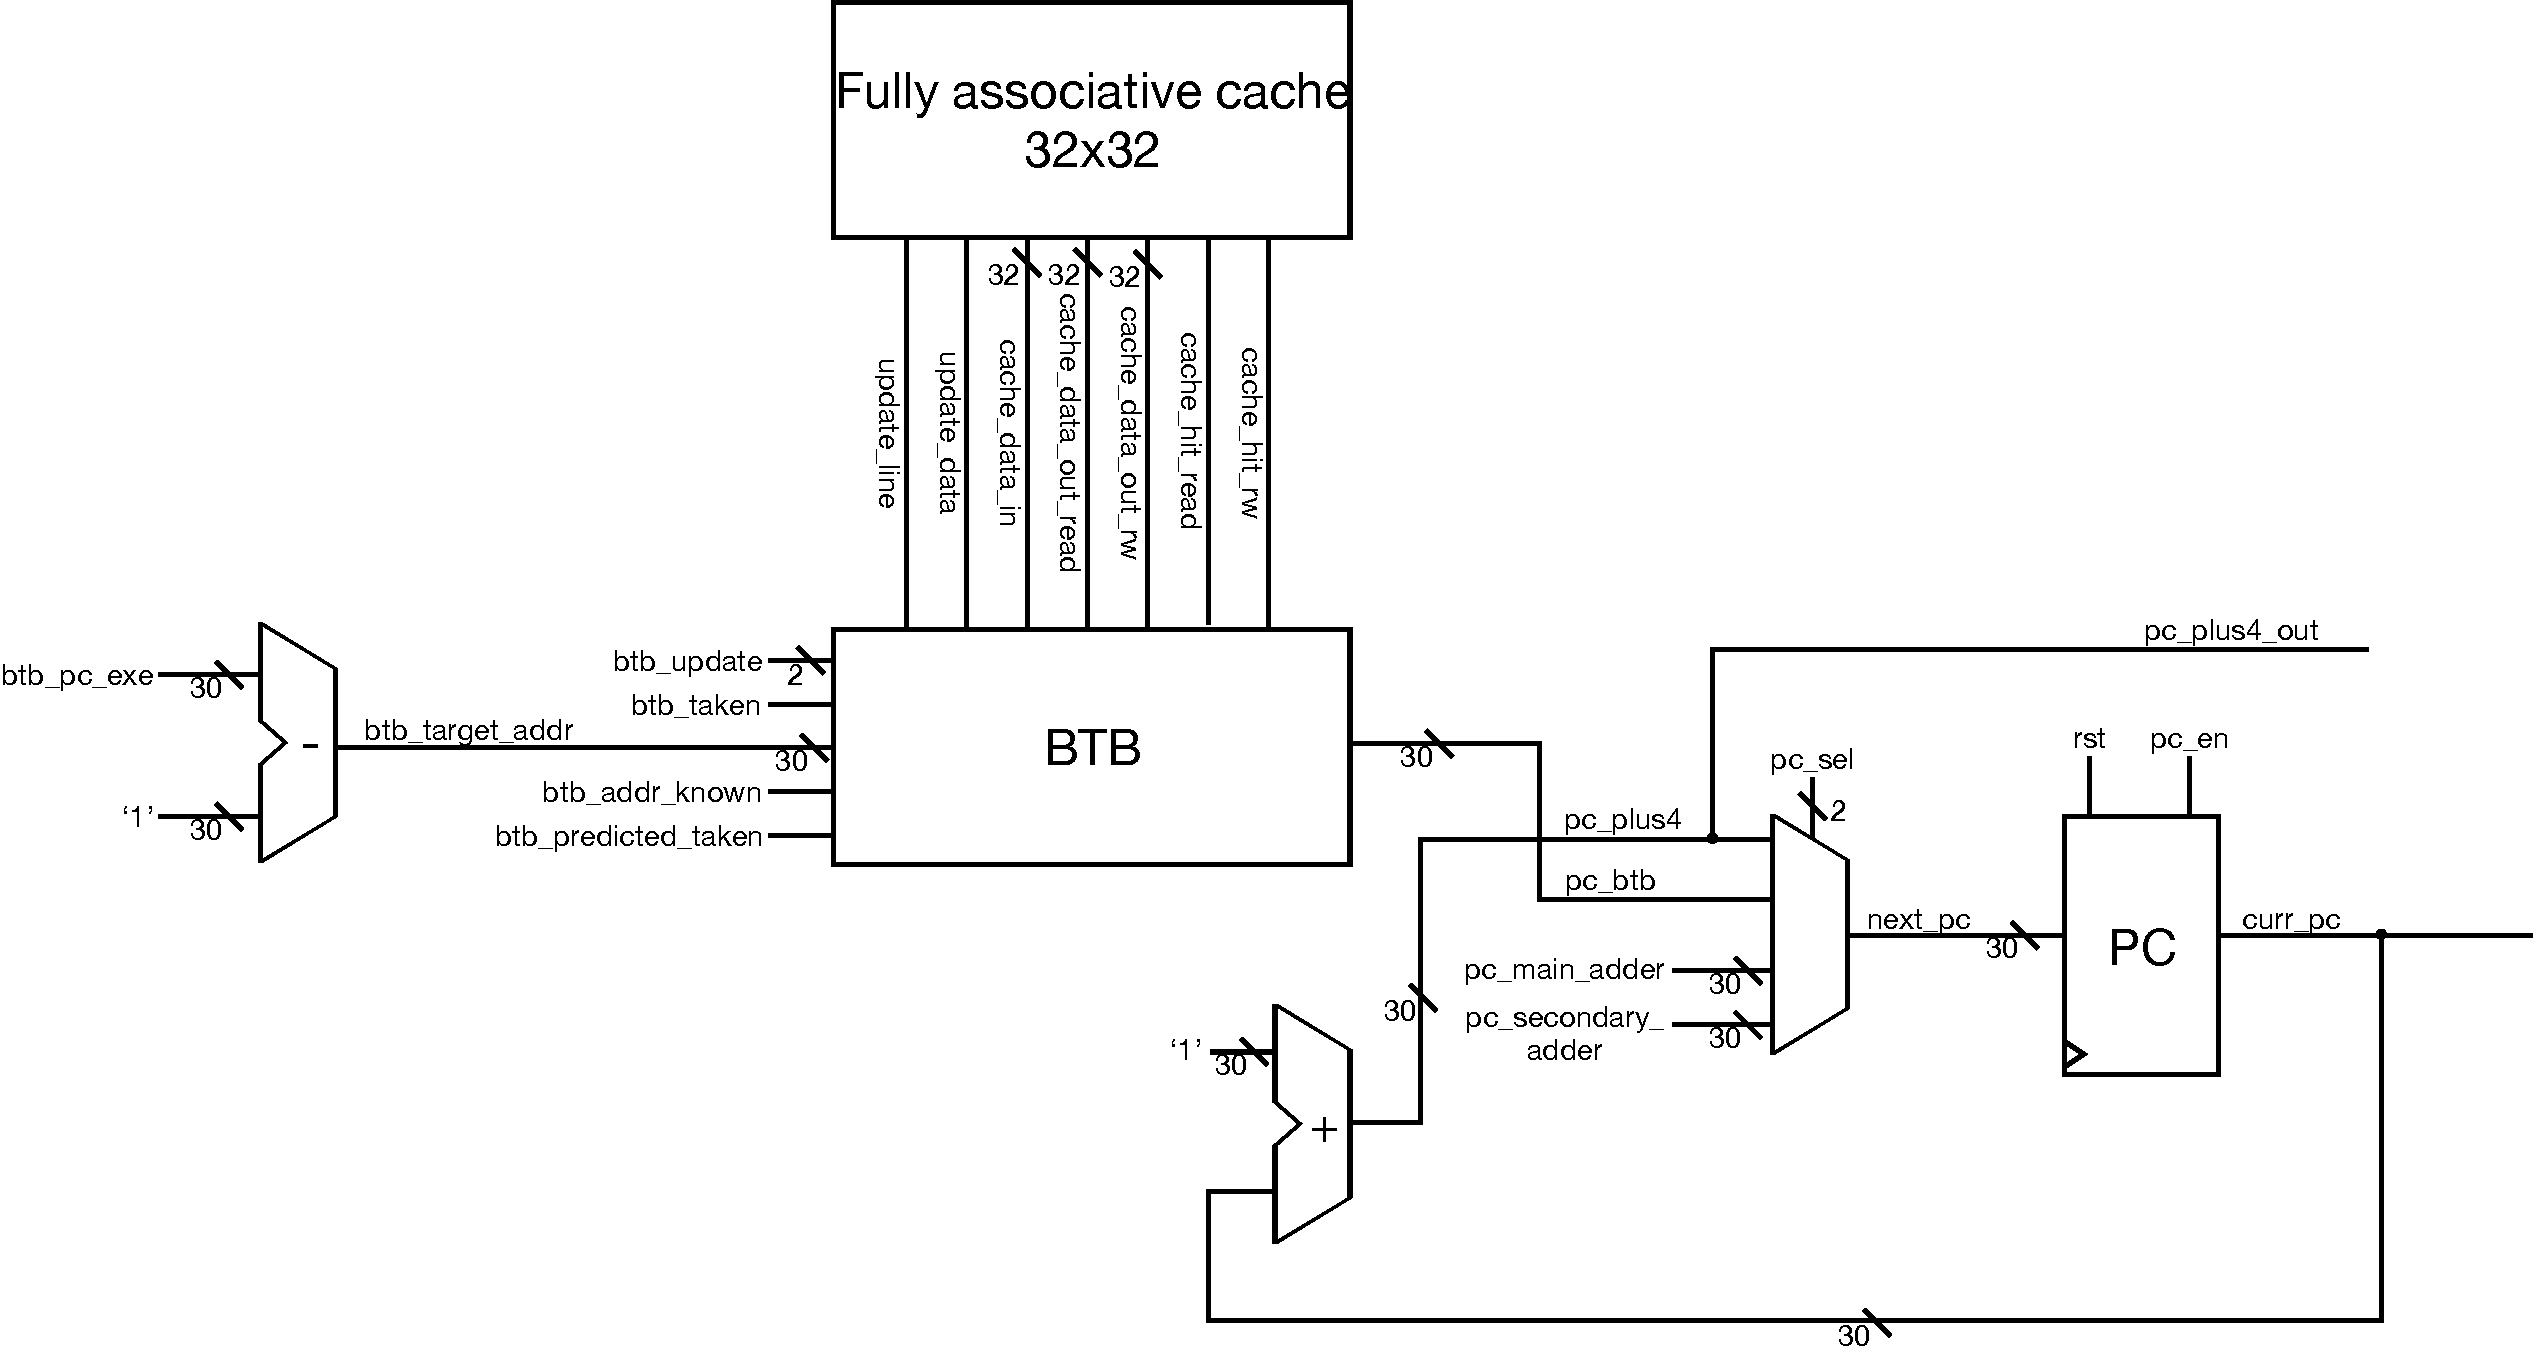
\includegraphics[width=\linewidth]{./chapters/figures/IF_stage.pdf}
	\caption{Block diagram of the IF stage}
	\label{fig:IF_stage}
\end{figure}

There are:

\begin{enumerate}
    \item a register storing the value of the current PC.
    \item A mux that selects among its 4 inputs which will be the next PC value.
    \item An adder that calculates $current\ pc + 4$
    \item A {\it Branch Target Buffer} (BTB) able to recognize and predict the behavior of known branches and jumps
    \item A 32-entries, 32 bits, fully associative cache that it is used by the BTB to recognize known branches and jumps
    \item A subtractor calculating $btb\ pc\ exe - 4$, that is the PC of the instruction in the EXE stage. It is used when updating the BTB content.
\end{enumerate}

In this stage the PC is used on 30 bits instead of 32 because instructions are aligned on 32 bits boundaries, therefore the 2 LSBs are always 0
and it was useless to add more HW to handle them.

\section{Branch Target Buffer}

The {\it branch target buffer} is a hardware structure used to known in the IF stage if the instruction being fetched is a known branch or jump.
It does so by accessing in read mode its cache using as address the current pc (this connection is not shown in figure \ref{fig:IF_stage}). For the differences
between read mode and write mode of the cache refer to subsection \ref{subsec:fully_cache}.
Our BTB operates over 3 values, as shown in figure \ref{fig:BTB_fields}.

\begin{figure}[!ht]
    \centering
    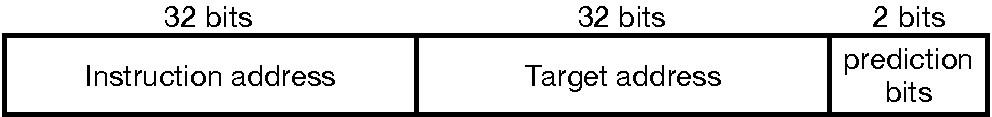
\includegraphics[width=\linewidth]{./chapters/figures/BTB_fields.pdf}
	\caption{Branch target buffer values}
	\label{fig:BTB_fields}
\end{figure}

\begin{enumerate}
    \item The {\it instruction address} is the memory address where the instruction resides. In our implementation corresponds to the TAG value in the cache.
    \item The {\it target address} is where the PC branch or the jump would go in case the jump condition is verified.
    \item The {\it prediction bits} are used by the FSM inside the BTB to predict whether a branch will be taken or not. The state machine of the prediction bits is shown in figure \ref{fig:BTB_FSM}.
\end{enumerate}

The target address, concatenated with the prediction bits, form a 32 bit value which corresponds to the data stored inside the cache.\\
Now let's take a closer look to the FSM implementation.

\begin{figure}[!ht]
	\centering
	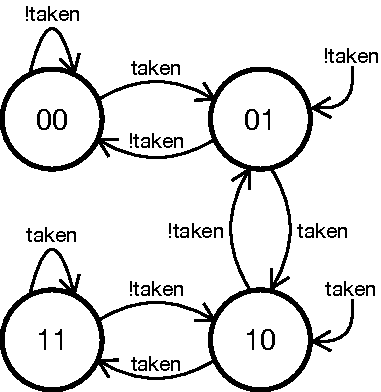
\includegraphics[width=0.3\linewidth]{./chapters/figures/BTB_FSM.pdf}
    \caption{Branch target buffer FSM representation}
    \label{fig:BTB_FSM}
\end{figure}

There are two entry points in the FSM: one that enters the state \verb|01| and one that enters the state \verb|10|. The former is used to add a new branch as non-taken,
while the latter is used for the opposite. In the delivered implementation only the {\it taken} entry point is used, but since at the beginning of the development we did not
know if we would have added also non-taken branch to the BTB, we felt that this degree of flexibility would have been nice to have.

Besides this particular, the FSM is straightforward: the 2 bits are used to store the state of a branch, and their values have the following meanings:

\begin{enumerate}
    \item \verb|00|: strongly not taken.
    \item \verb|01|: weakly not taken.
    \item \verb|10|: weakly taken.
    \item \verb|11|: strongly taken.
\end{enumerate}

The value of \verb|btb_taken| is 0 for the first two cases and 1 for the last two, provided that the address that is being considered is known to the cache (that is, we have $hit = 1$ in read mode).

The BTB of course needs to be updated every time a branch is executed or discovered. This is achieved by writing in \verb|btb_update| \verb|01| to update only the history bits or \verb|10| to add a new
branch, by concatenating the target address to the history bits and by setting the cache's write address to the instruction's PC.

\subsection{Fully associative cache}
\label{subsec:fully_cache}

A key component of the BTB is the cache, where as already said all the known branches and jumps are stored. We decided to use a 32-entries fully associative cache to have the highest possible hit rate,
since every miss could hurt the pipeline's performance. Its general, simplified structure is shown in figure \ref{fig:BTB_cache}.

\begin{figure}[!ht]
	\centering
	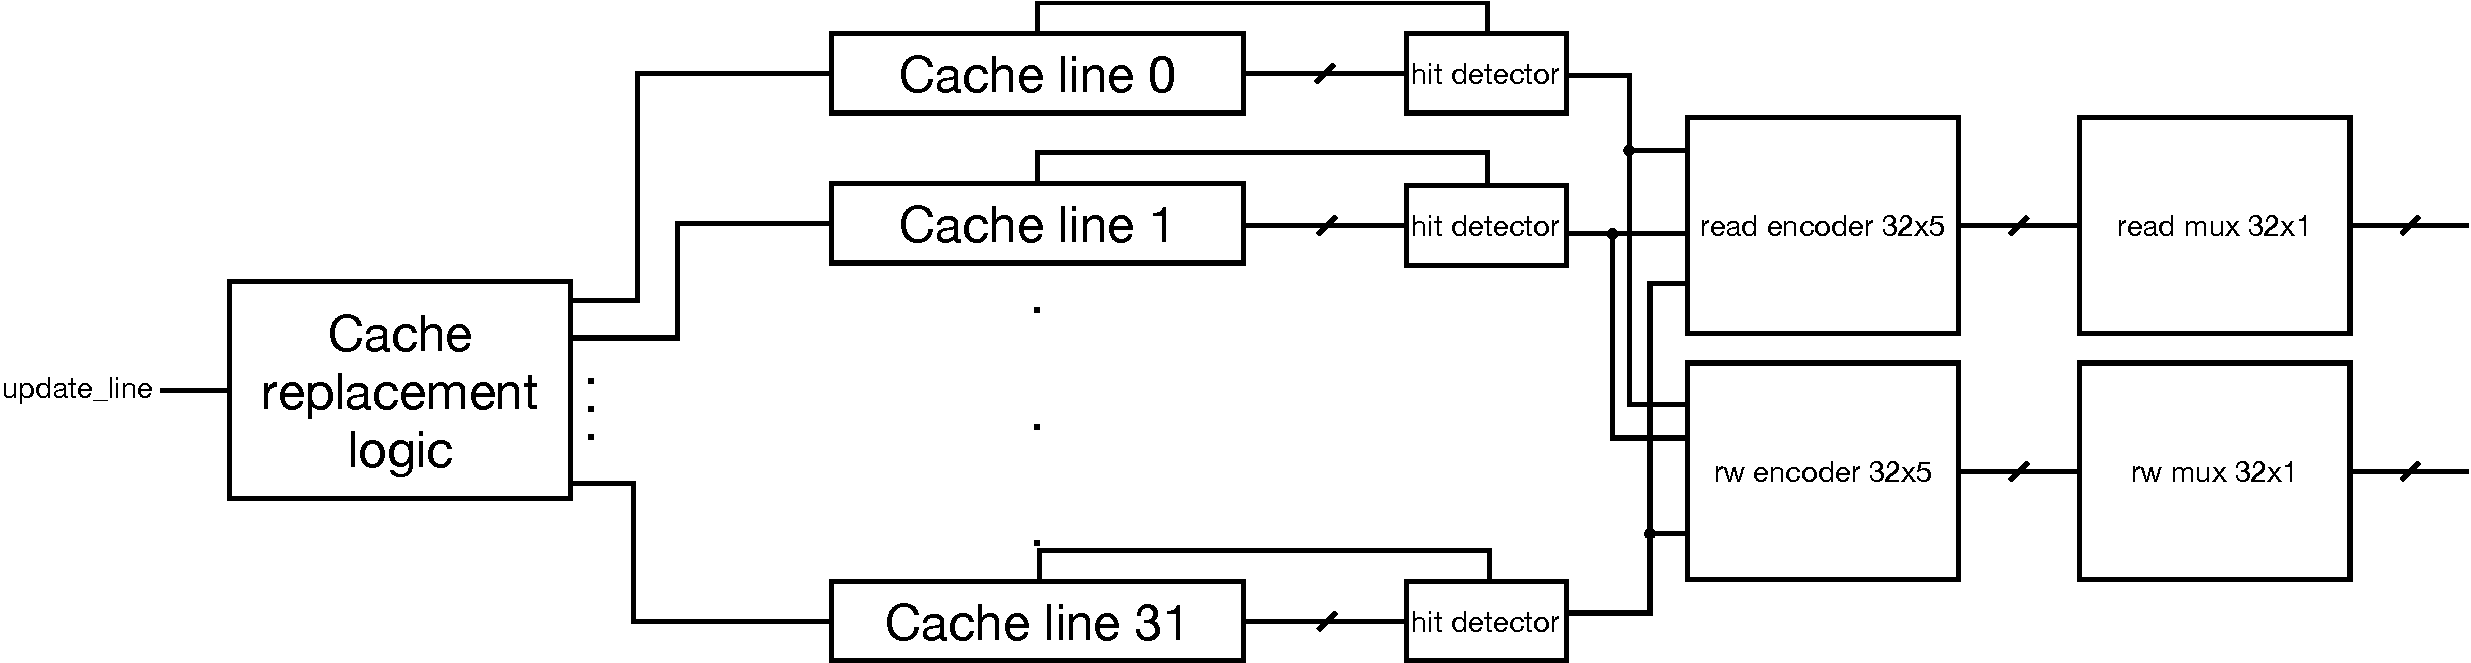
\includegraphics[width=\linewidth]{./chapters/figures/BTB_cache.pdf}
    \caption{Cache general representation}
    \label{fig:BTB_cache}
\end{figure}

This cache support two read operations and a write operation per clock cycle and implements a FIFO replacement logic. Each cache line has a hit detector, which is used to detects a hit in case of a read, and
to issue a line update (only the data is updated, not the tag) if requested by the BTB. The hits signals then enter two 32-entries encoders which in turn drive two 32-entries muxes, used to output the data from the cache.
To illustrate exactly how a cache line and a hit detector work we'll refer to picture \ref{fig:BTB_cache_line}.

\begin{figure}[!ht]
	\centering
	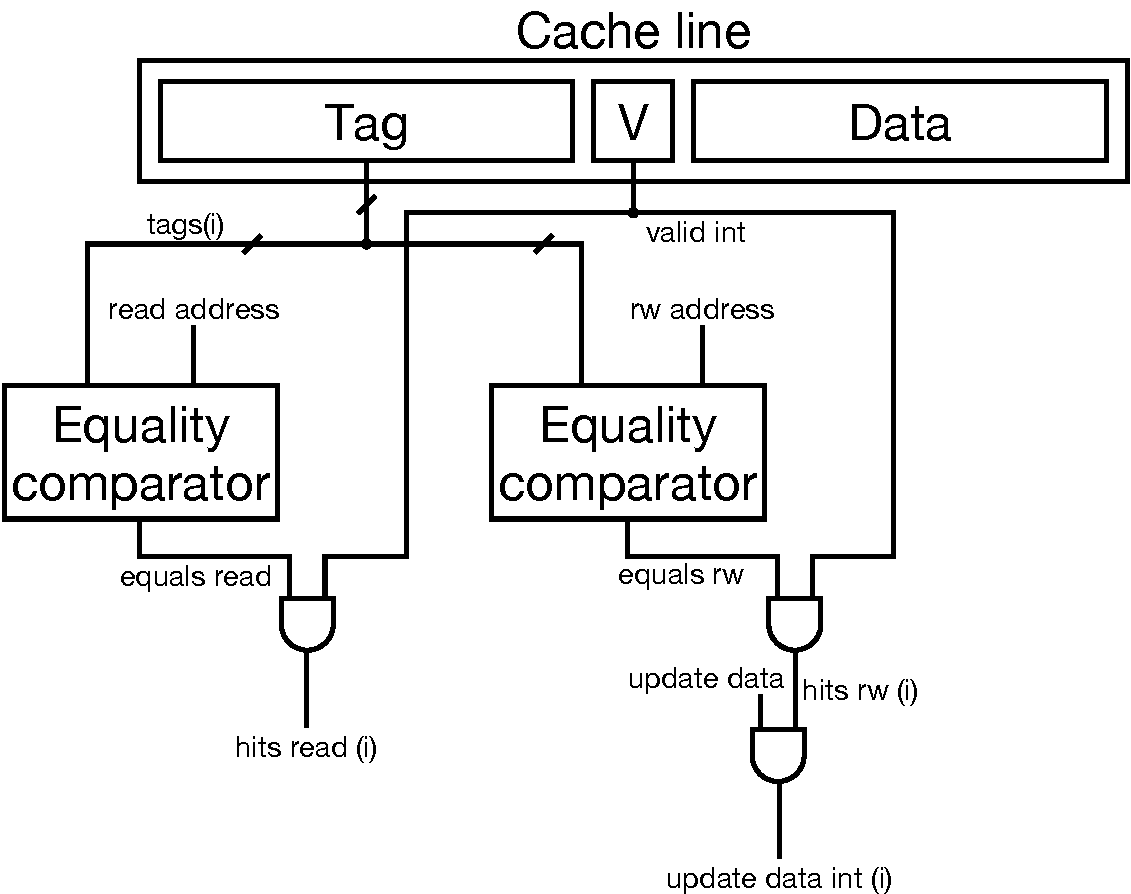
\includegraphics[width=0.6\linewidth]{./chapters/figures/BTB_cache_line.pdf}
    \caption{Cache line and hit detectors}
    \label{fig:BTB_cache_line}
\end{figure}

A cache line is composed of a 30 bits \verb|tag| field, that stores the PC of the branch/jump, a validity bit used to discriminate invalid data after a reset and a 32 bits \verb|data| field that keeps the value
of the target address along with the history bits. The tag enter two equality comparators to check if a match exists either with the read address, the write address, or both. To determine if a hit has occurred this
is not sufficient though, because the data stored in the tag may be invalid. To solve this issue an AND is executed between the validity bit and each comparator's output. The write part has an additional AND between
its hit value and the \verb|update_data| signal to determine if this line have to update its \verb|data| field.

\section{Program counter selection}

There are 4 possible next program counter values to choose at each clock cycle:
\begin{enumerate}
    \item $PC + 4$
    \item $PC_{BTB}$
    \item $PC_{main\ adder}$
    \item $PC_{secondary\ adder}$
\end{enumerate}

$PC + 4$ is the default choice when the BTB doesn't recognize the address and the EXE have not executed a branch or a jump. $PC_{BTB}$ is taken whenever the BTB recognizes the address and the EXE have not executed
any branch or jump. $PC_{main\ adder}$ is used when the EXE have executed a \verb|jr| or \verb|jalr|. Finally, $PC_{secondary\ adder}$ is the value used when any branch or jump except \verb|jr| and \verb|jalr| is
executed in the EXE stage.
\chapter{ID stage}
\label{chap:id}

In the ID stage instructions are decoded and the register file is accessed. Its block diagram is shown in picture \ref{fig:ID_stage}

\begin{figure}[!ht]
	\centering
	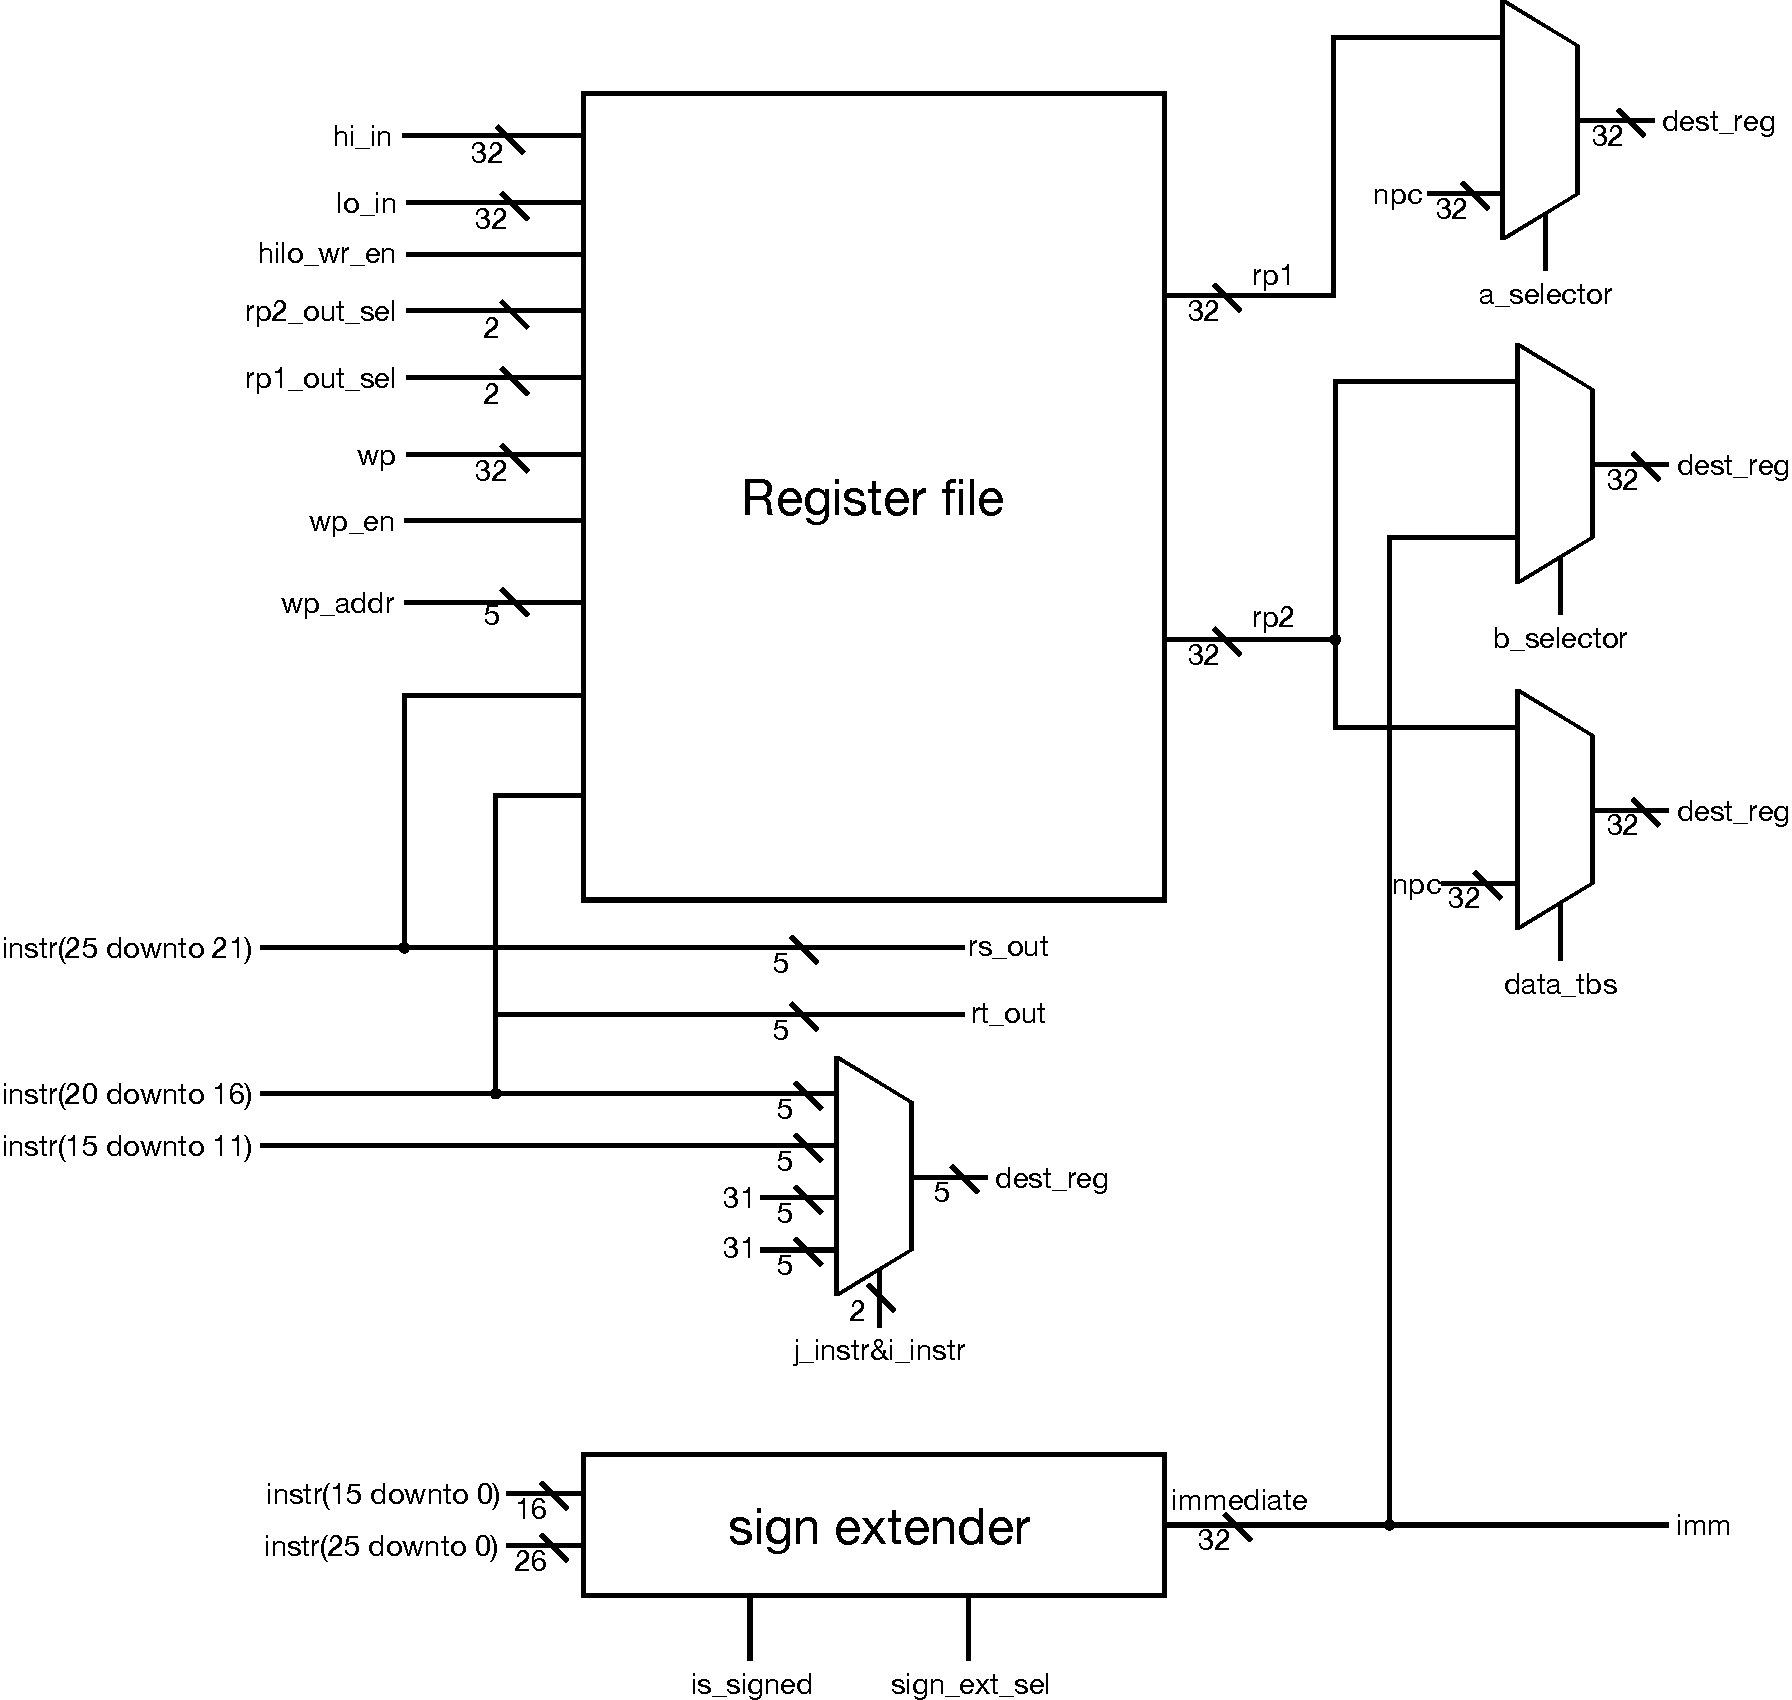
\includegraphics[width=.6\linewidth]{./chapters/figures/ID_stage.pdf}
	\caption{Block diagram of the ID stage}
	\label{fig:ID_stage}
\end{figure}

\section{Register file}

The {\it register file} is one of the two main components in this stage. It has 2 read ports and 3 write ports, although a write operation never use all of them at the same time.
It contains 32 {\it general purpose registers} (GPR), as stated by the ABI, and 2 additional registers called \verb|lo| and \verb|hi|, accessible only by special instructions and used
to store multiplications' results. Among the GPR there is a special register, the register number 0, that cannot be written and always contains the value \verb|0x00000000|.
The full list of the ABI-compliant registers is shown in table \ref{tab:registers}:

\begin{table}[!ht]
    \centering
    \begin{tabular}{ |c|c|c|c| }
        \hline
        Name & Number & Use & Directly accessible \\

        \hline
        \verb|$zero| & 0 & constant 0 & Yes \\
        \hline
        \verb|$at| & 1 & assembler temporary & Yes \\
        \hline
        \verb|$v0-$v1| & 2-3 & values for function returns and expression evaluation & Yes \\
        \hline
        \verb|$a0-$a3| & 4-7 & function arguments & Yes \\
        \hline
        \verb|$t0-$t7| & 8-15 & temporaries & Yes \\
        \hline
        \verb|$s0-$s7| & 16-23 & saved temporaries & Yes \\
        \hline
        \verb|$t8-$t9| & 24-25 & temporaries & Yes \\
        \hline
        \verb|$k0-$k1| & 26-27 & reserved for OS kernel & Yes \\
        \hline
        \verb|$gp| & 28 & global pointer & Yes \\
        \hline
        \verb|$sp| & 29 & stack pointer & Yes \\
        \hline
        \verb|fp| & 30 & frame pointer & Yes \\
        \hline
        \verb|$ra| & 31 & return address & Yes \\
        \hline
        \verb|$lo| & 32 & stores the lower 32 bits of a multiplication & No \\
        \hline
        \verb|$hi| & 33 & stores the higher 32 bits of a multiplication & No \\
        \hline
    \end{tabular}
    \caption{DLX registers. Taken from \cite{abi_regs}}
    \label{tab:registers}
\end{table}

In the ID stage the RF is accessed in read, since it is the WB stage to access it in write. To select the registers the bits 25-21 and 20-11 are used,
because they represent the \verb|rs| and \verb|rt| fields in an R instruction. These values are not the only ones used by the RF to decide which values
its read ports should take: as illustrated in table \ref{tab:registers}, there are two non-directly accessible registers, \verb|lo| and \verb|hi|. To perform
the final output selection two control signals are used, \verb|rp1_out_sel| and \verb|rp2_out_sel|, that drive 2 internal muxes that choose the value of the read ports as follows:

\begin{enumerate}
    \item \verb|00|: output the selected GP register.
    \item \verb|01|: output the \verb|lo| register.
    \item \verb|10|: output the \verb|hi| register.
    \item \verb|11|: output \verb|0x00000000|.
\end{enumerate}

\section{Sign extender}

This component is used by I and J instructions to extend their immediate fields on 32 bits. In fact, I instructions have their immediate stored in the lower 16 bits of the instruction,
while the J have it stored on the lower 26 bits. Moreover, these bits could represent a signed or unsigned value, like in the case of a \verb|addi| and a \verb|addui|, therefore this
has to be taken in account during the extension. As shown in figure \ref{fig:ID_stage}, two controls signals enter the sign extender: \verb|is_signed| and \verb|sign_ext_sel|. The former
is used to extend either with 0s or taking into account the sign, while the latter is used to decide if the extension should consider only 16 bits or 26.

\section{Selection muxes}

In the rightmost part of figure \ref{fig:ID_stage} 3 muxes 2x1 can be seen. In a standard MIPS pipeline these would reside in the EXE stage, but since it is the slowest stage of the pipeline
we decided to shorten its critical path by bringing them in the ID stage. The first mux is used to select between the read port 1 of the RF and the program counter coming from the stage before,
while the second mux chooses among the RF's read port 2 and the immediate value coming from the sign extender. The output of these two muxes form respectively the \verb|a| and \verb|b| inputs
of the EXE stage. The third mux is used to select the output of the RF's read port 2, which is the data that would go inside the memory when executing a store, and the npc, that is used to execute
in a single cycle a \verb|jalr| instruction.
\chapter{EXE stage}
\label{chap:exe}
\chapter{MEM stage}
\label{chap:mem}

In this stage memory is read during a load and it is written during a store. Its block scheme is shown in figure \ref{fig:MEM_stage}.

\begin{figure}[!ht]
	\centering
	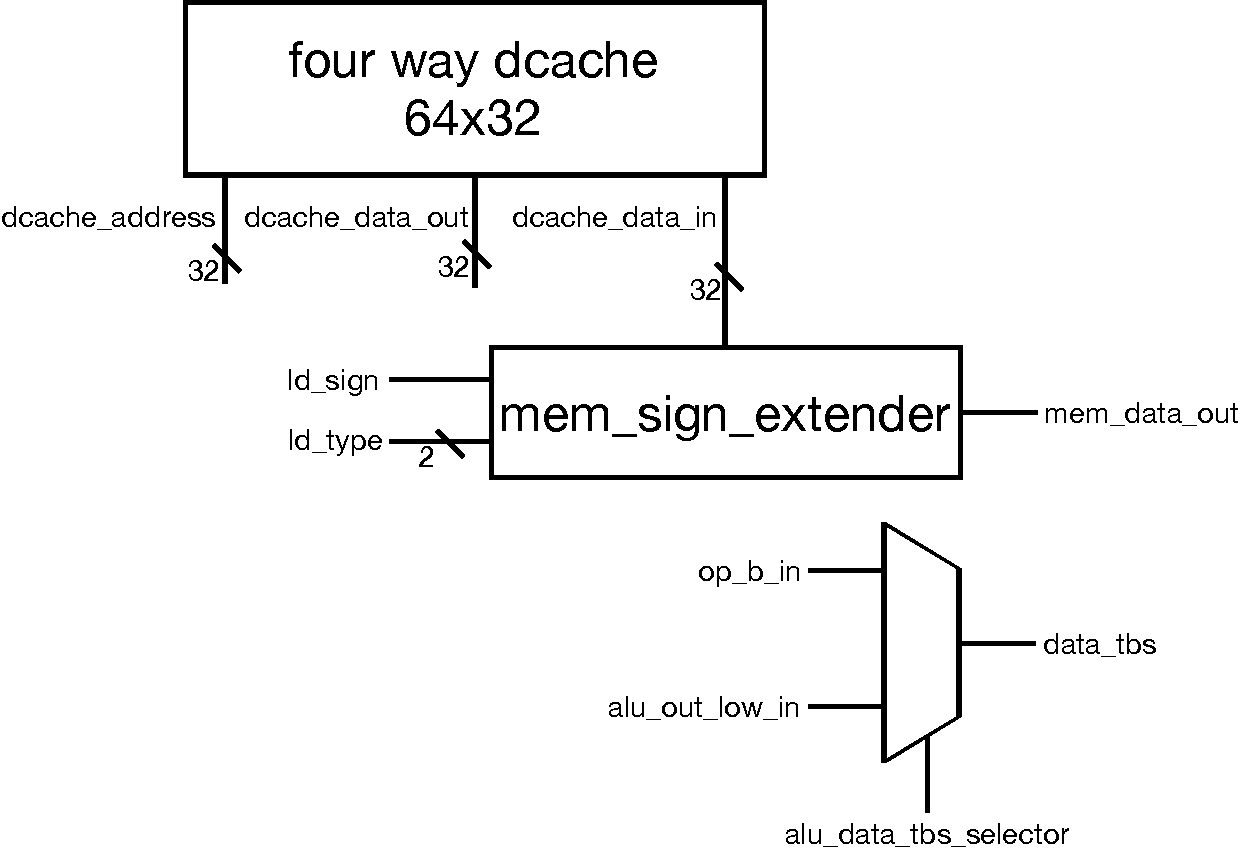
\includegraphics[width=.7\linewidth]{./chapters/figures/MEM_stage.pdf}
	\caption{Block diagram of the MEM stage}
	\label{fig:MEM_stage}
\end{figure}

The lowest mux is used when in the MEM stage an operation different from a load and a store is executed. It selects \verb|alu_out_low_in| when in the RF the data coming from the ALU
must be stored, otherwise it selects \verb|op_b_in|, used by \verb|jalr| and \verb|jal| instruction to save in the RF the value of the program counter.

\section{Data cache}

The main datapath component of this stage is the data cache. It is a 64-entries four-way associative cache, able to perform two reads, two writes, or one read and one write per clock cycle.
This is due to the fact that the cache has two interfaces, one connected to the processor and another one connected to the memory controller. In figure \ref{fig:dcache} it is shown
the block diagram for the processor's side.

\begin{figure}[!ht]
	\centering
	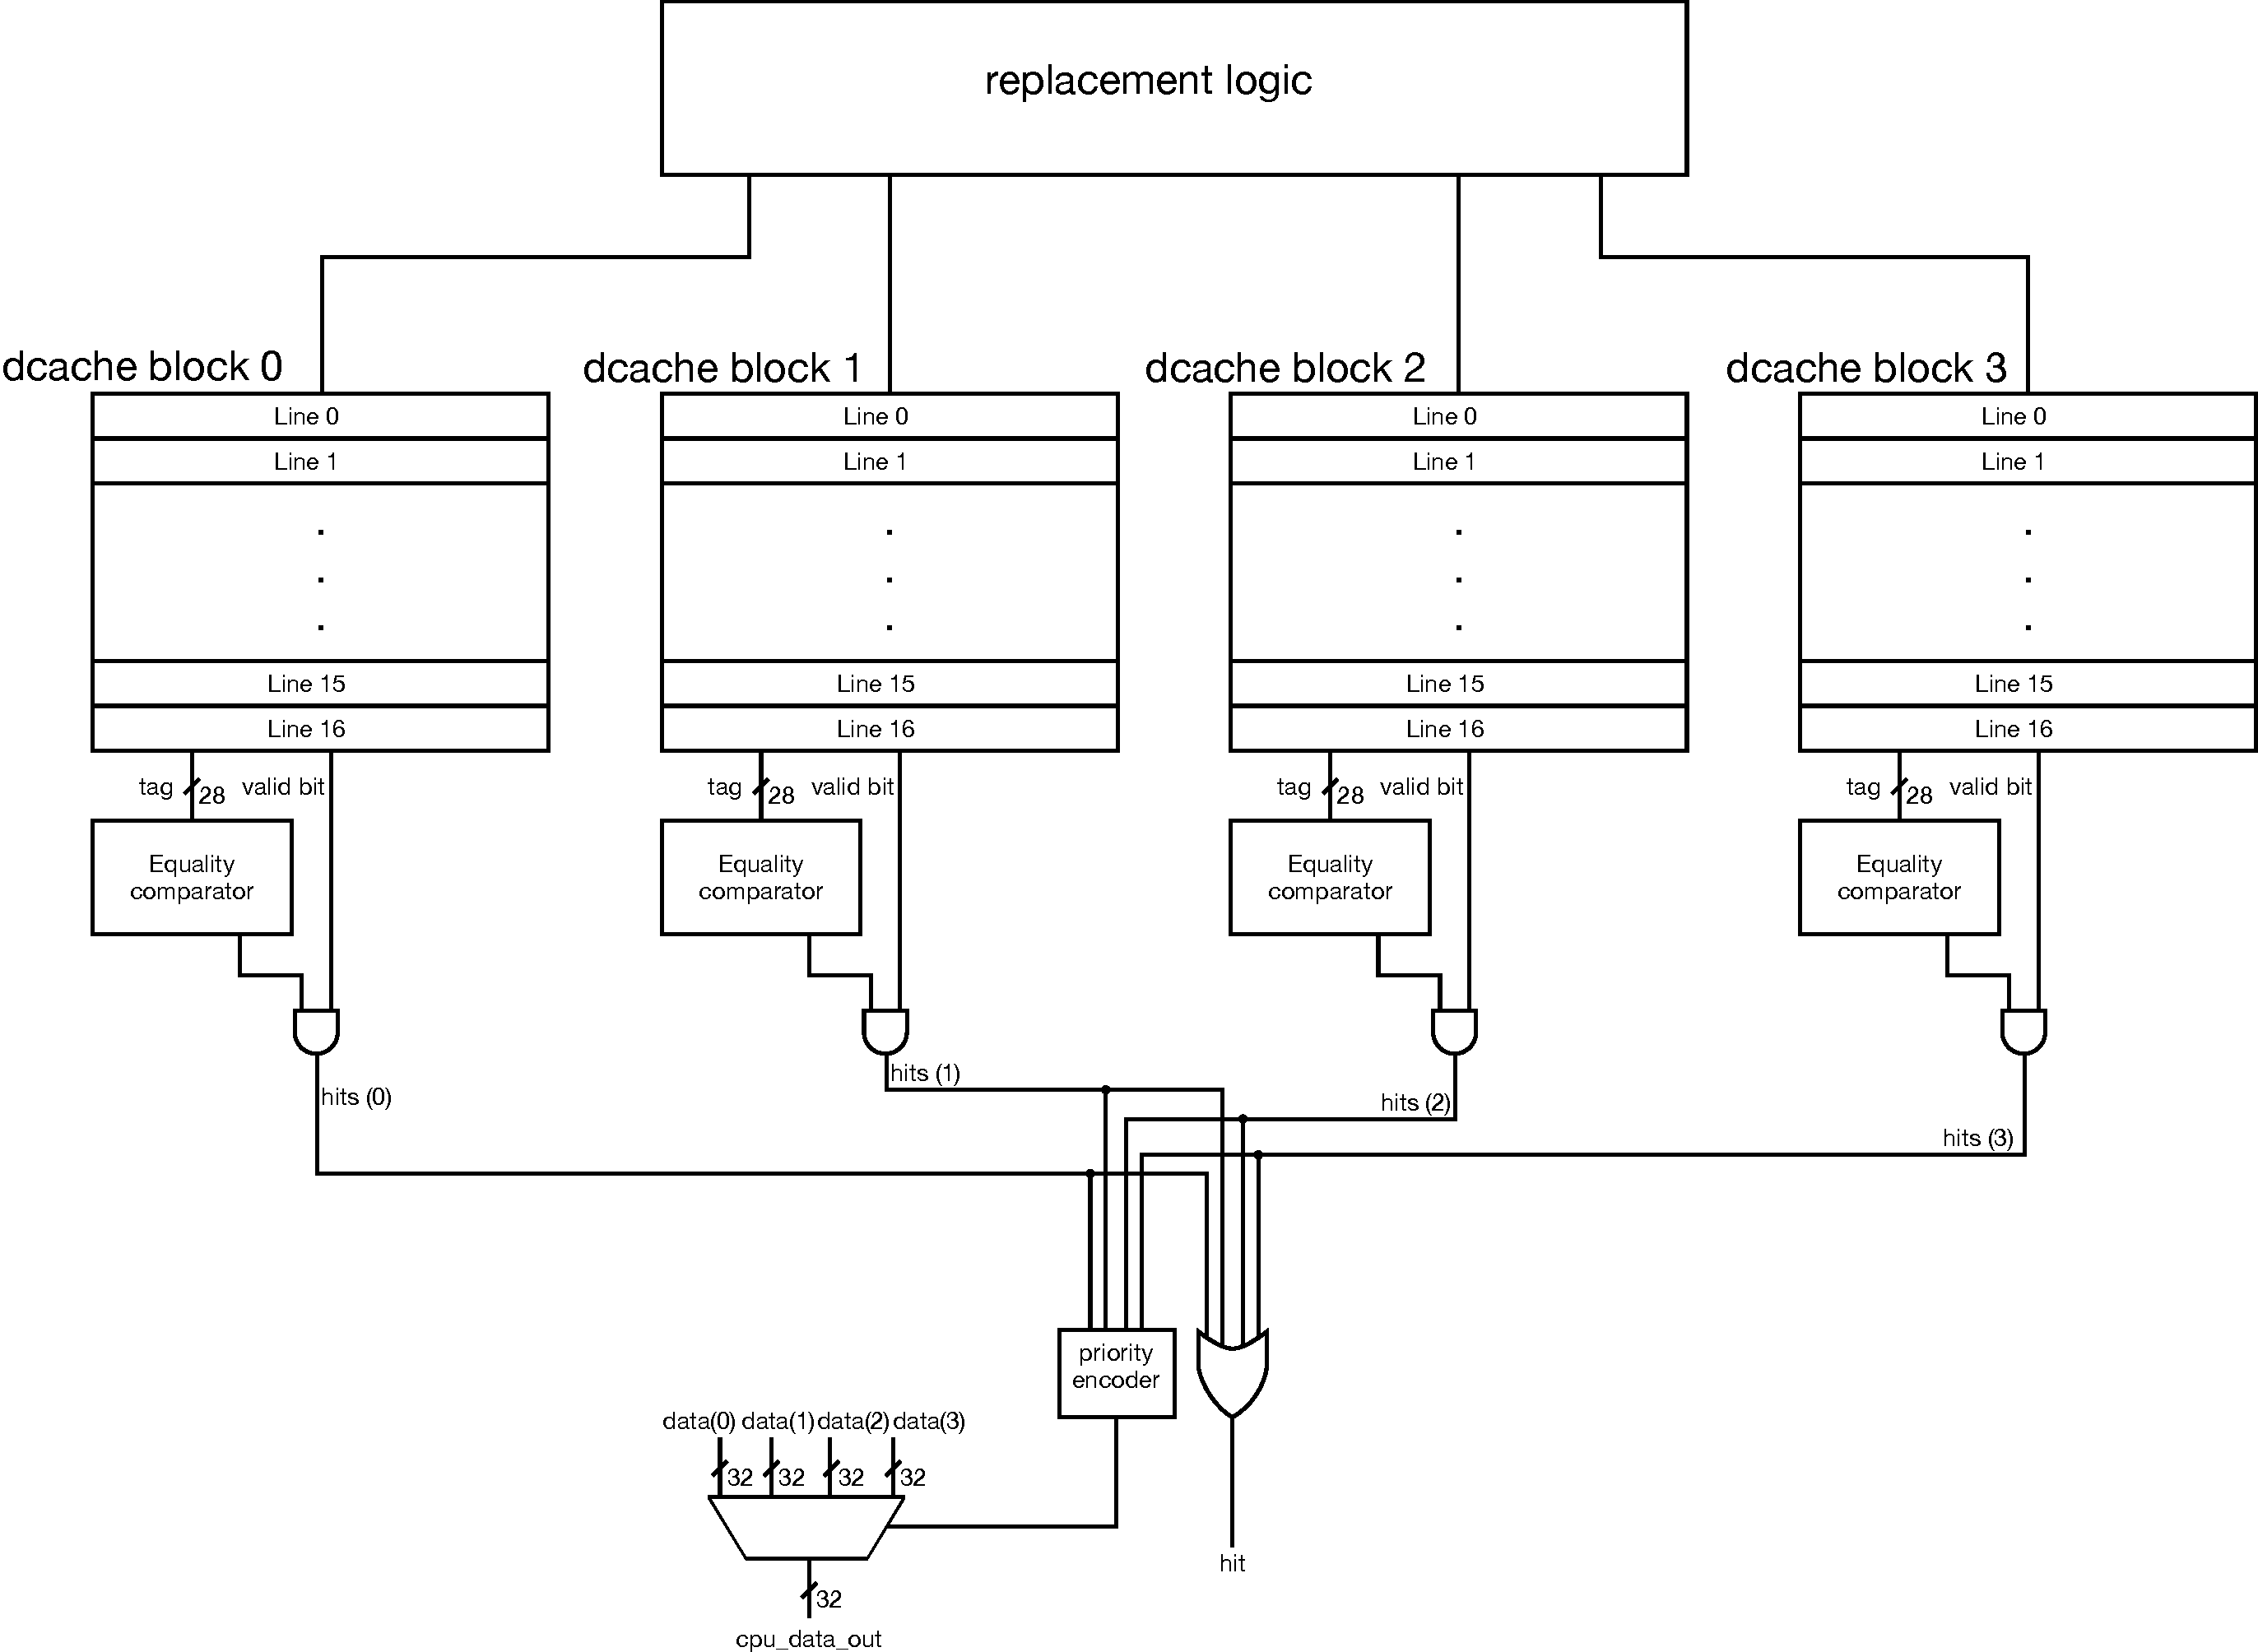
\includegraphics[width=\linewidth]{./chapters/figures/dcache.pdf}
	\caption{Dcache's processor side}
	\label{fig:dcache}
\end{figure}

As it can be seen, the cache's lines are divided among four blocks. Each line in a block corresponds to a different set, therefore a set is formed by considering all the lines having the same
number. The structure of the line is the same as the one shown in figure \ref{fig:BTB_cache_line}, but with a difference: if the data being stored comes from the CPU it is saved in big endian.
In fact, the DLX is expected to work in big endian, therefore every time data comes out the CPU it must do so in this format. To reuse some modules we already had, however, we preferred to internally
work in little endian. We've identified the cache as the best place to perform DLX-RAM data conversion transparently.

Moving on, each block has its own logic to detect if the line corresponding to the chosen set is generating a hit. The detection logic works in the same way as in the fully associative cache explained in section
\ref{subsec:fully_cache} and will not be discussed again. The four hits signal generated by the blocks then enter a priority encoder, which generate a suitable encoding for the data mux. Moreover, these signals
converge into a 4-inputs OR gate that outputs the final \verb|hit| signal.

\subsection{Replacement logic}

On top of the cache's blocks there is the replacement logic, shown in figure \ref{fig:dcache_replacement}.

\begin{figure}[!ht]
	\centering
	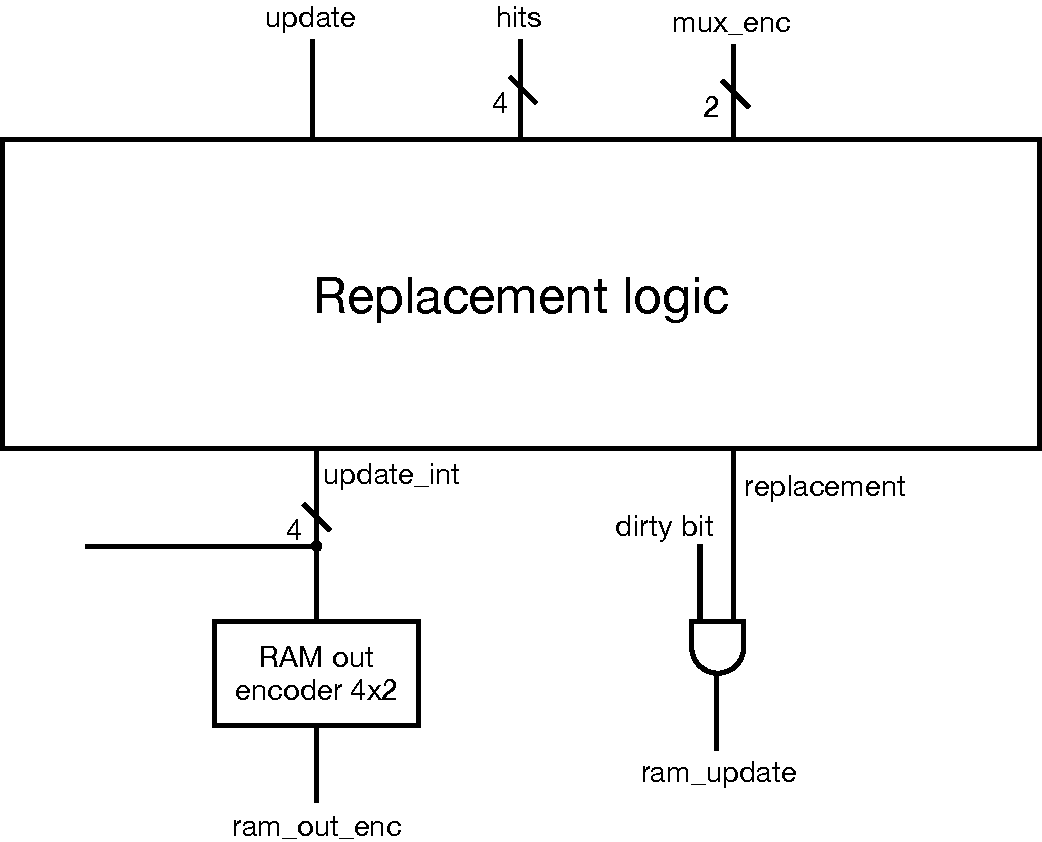
\includegraphics[width=0.6\linewidth]{./chapters/figures/dcache_replacement.pdf}
	\caption{Replacement logic}
	\label{fig:dcache_replacement}
\end{figure}

This unit receives in feedback the \verb|hits| signal generated by the four blocks and the encoding value for the data mux, moreover receives either from the memory controller or the control unit
an update signal. These information are combined together to decide how and if to update or replace the data contained in the cache.
When an update is requested for data not present yet in the cache and there are free blocks, a FIFO scheme is used and both \verb|replacement| and \verb|dirty_bit| are low.
On the other hand, when an update is requested for data already known to the cache, \verb|ram_out_enc| forwards the value of the input \verb|mux_enc| and it keeps \verb|replacement| low.
However, if new data must be written and there's no room in the blocks, an eviction must be performed. In this case the signal \verb|replacement| is raised to 1. Also the \verb|dirty_bit| is set to 1
since we are considering the case in which all the blocks are used. Hence, the AND goes to 1 and the both the control unit and the memory controller receive it.
For the explanation of how cache eviction and cache misses are handled please refer to section \ref{sec:cache_handling}.

\section{Sign extender}

The DLX, as seen in table \ref{tab:sup_instr}, supports many types of load operation: with or without sign extension, and on different sizes of data. The job of the sign extender is therefore the one
of taking in input the data read from the cache and to extend it properly (if necessary). It is driven by the control unit through the \verb|ld_sign| and \verb|ld_type| signals. The former is set to 0
when load is unsigned, to 1 when it is signed. The latter is a 2-bit signals that specifies from where 0-extension or sign-extension should take place. The possible values are:

\begin{enumerate}
    \item \verb|00|: use 32 bits. In this case no operation is performed on the incoming data.
    \item \verb|01|: use 16 bits.
    \item \verb|10|: use 8 bits.
    \item \verb|11|: reserved. In this particular implementation it works in the same way as \verb|00|.
\end{enumerate}
\chapter{WB stage}
\label{chap:wb}

This is the last stage of the pipeline. It is conceptually part of the ID stage since it drives the write signals of the register file.
It is composed only by a 2x1 mux, which decides the value of the \verb|wp| port of the register file shown in figure \ref{fig:ID_stage}.
The choice is made among the data read from the cache in the MEM stage or the one coming from a calculation performed in the EXE stage.
It also drives:

\begin{enumerate}
    \item \verb|wp_en|, set to 1 when an operation has to store data in a GP register.
    \item \verb|hilo_wr_en|, set to 1 when the result of a multiplication has to be stored in \verb|lo| and \verb|hi|.
    \item \verb|wp_addr|, which is the value of the destination register.
\end{enumerate}
\chapter{Control Unit}
\label{chap:cu}

The DLX's control unit is mainly based on the hardwired approach, although some operations are handled by in-stage FSMs. The former approach has been chosen
because most of the control signals of an operation never changes during its execution. For example, for an \verb|add| instruction the value of \verb|rp1_out_sel|
is always \verb|00| and will never change, no matter what happens in the pipeline. Because of this, reading the values from a control register and writing them directly in the
component is the fastest and cheapest way to control the datapath. However, not all the signals can be known a-priori, or they need to change over time to handle complex operations:
the former case is represented by the forwarding signals for example, while the latter from the multiplication. Due to this we had to resort to in-stage FSM able to correctly manage
these situations.

The control unit is by far the most complex component in the DLX, therefore to ease the explanation the rest of the chapter is divided in sections, each of which explains what happens
in the related stage. 

\section{IF stage}
\label{sec:cu_IF_stage}

The PC register in the datapath is used to access the {\it instruction ROM}, or IROM, where all the instructions to be executed are stored. The IROM's output is then sent to both the
control unit, to analyze the instruction's {\it opcode} and {\it func} fields, and to the IF/ID registers for decoding the rest of the fields in the ID stage.
The control units hosts two ROMs: one contains all the control words (also referred to as {\it CW}) related the I and J instructions, while the other one stores all the CW belonging
to the R instructions. The former is accessed using the opcode field, the latter using the func field. This distinction had to be done because all R instructions have the same opcode,
which is equal to \verb|0x00|.

\begin{figure}[!ht]
	\centering
	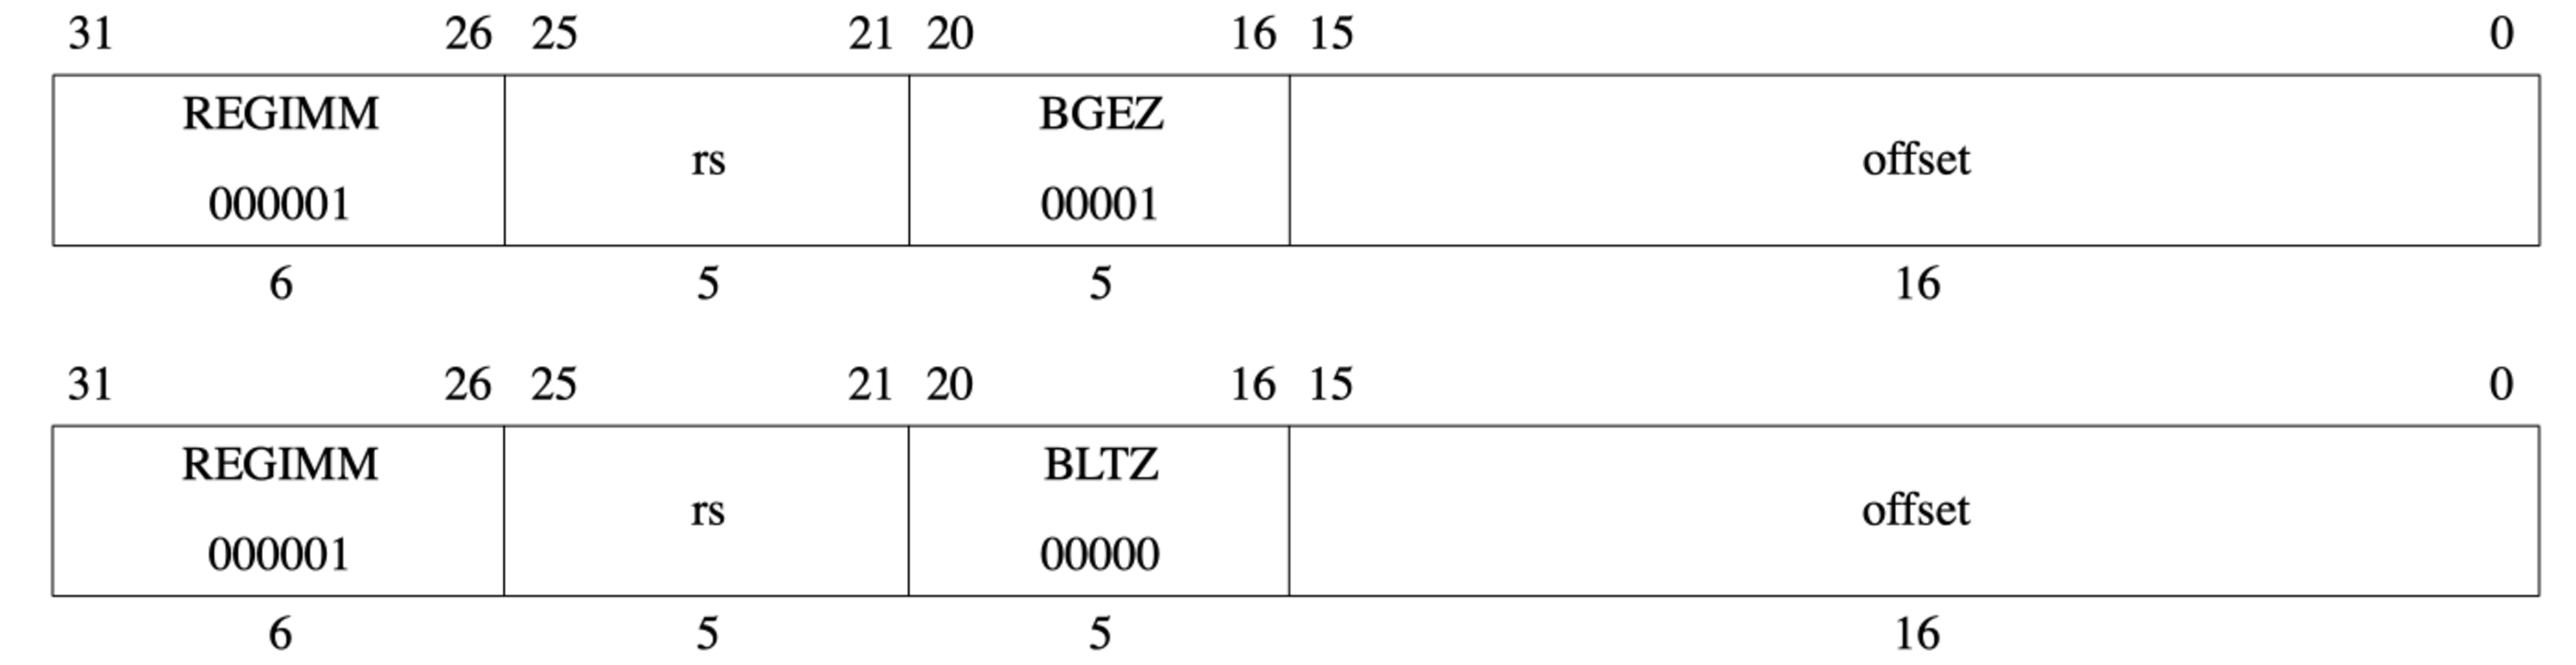
\includegraphics[width=\linewidth]{./chapters/figures/bltz_bgez.pdf}
    \caption{bltz and bgez instruction format. Taken from \cite{MIPS64_arch}}
    \label{fig:bltz_bgez}
\end{figure}

The control unit recognize this pattern and it chooses the right CW for each instruction. Nonetheless this is not the only particular case. As already shown in table \ref{tab:sup_instr},
\verb|bgez| and \verb|bltz| shares the same opcode. Their difference reside in the bits 20-16, which are set to \verb|00001| for the former, to \verb|00000| for the latter (figure \ref{fig:bltz_bgez}).
This information cannot be used to differentiate the branches directly in the CW's ROM, hence their final CW is generated dynamically.

This part of the control unit also decide from which source must come the next value of the PC register. Four cases have to be distinguished:

\begin{enumerate}
    \item The EXE stage have not executed a branch and the BTB predicts as not taken the current fetched instruction: in this case $PC + 4$ is chosen.
    \item The EXE stage have not executed a branch and the BTB predicts as taken the current fetched instruction: in this case $PC_{BTB}$ is chosen.
    \item The EXE has executed a \verb|jr| or a \verb|jalr|: the prediction of the BTB is discarded and $PC_{main\ adder}$ is chosen.
    \item the EXE has executed a branch or a jump different from \verb|jr| or \verb|jalr|: the prediction of the BTB is discarded and $PC_{secondary\ adder}$ is chosen.
\end{enumerate}

\section{ID stage}

The bits used to drive the ID stage are all static, therefore they are directly read from the control unit's IF/ID register and are sent to the datapath. Here is it worth commenting
how this stage interacts with the EXE stage. When a multiplication is in progress in the EXE stage it is the EXE stage's FSM to drive the ID/EXE registers, therefore all the ID's signals
going to the ID/EXE registers are set in high impedance to avoid conflicts.

The ID stage is also in charge of detecting a \verb|mult| instruction, and when it does so it may need to stall the pipeline. Unfortunately, when the multiplication's operand are sent to the
ID/EXE stage, they are automatically extended on 64 bits by the registers themselves. This means that a \verb|mult| cannot enters the EXE stage if one of its source operands is still being processed
in the pipeline. Due to this limitation, when an hazard is detected for a multiplication is detected, the control unit's ID stage in conjunction with the {\it stall unit} (explained in section \ref{sec:stall_unit})
stalls the IF and the ID stage, until all the data hazards have been resolved.

\section{EXE stage}
\label{sec:cu_exe_stage}

This is the biggest stage in the control unit's pipeline. It contains an FSM to handle the multiplication, which is the only instruction that requires more than a single clock cycle to execute.
Its state diagram is shown in figure \ref{fig:mul_fsm}.

\begin{figure}[!ht]
	\centering
	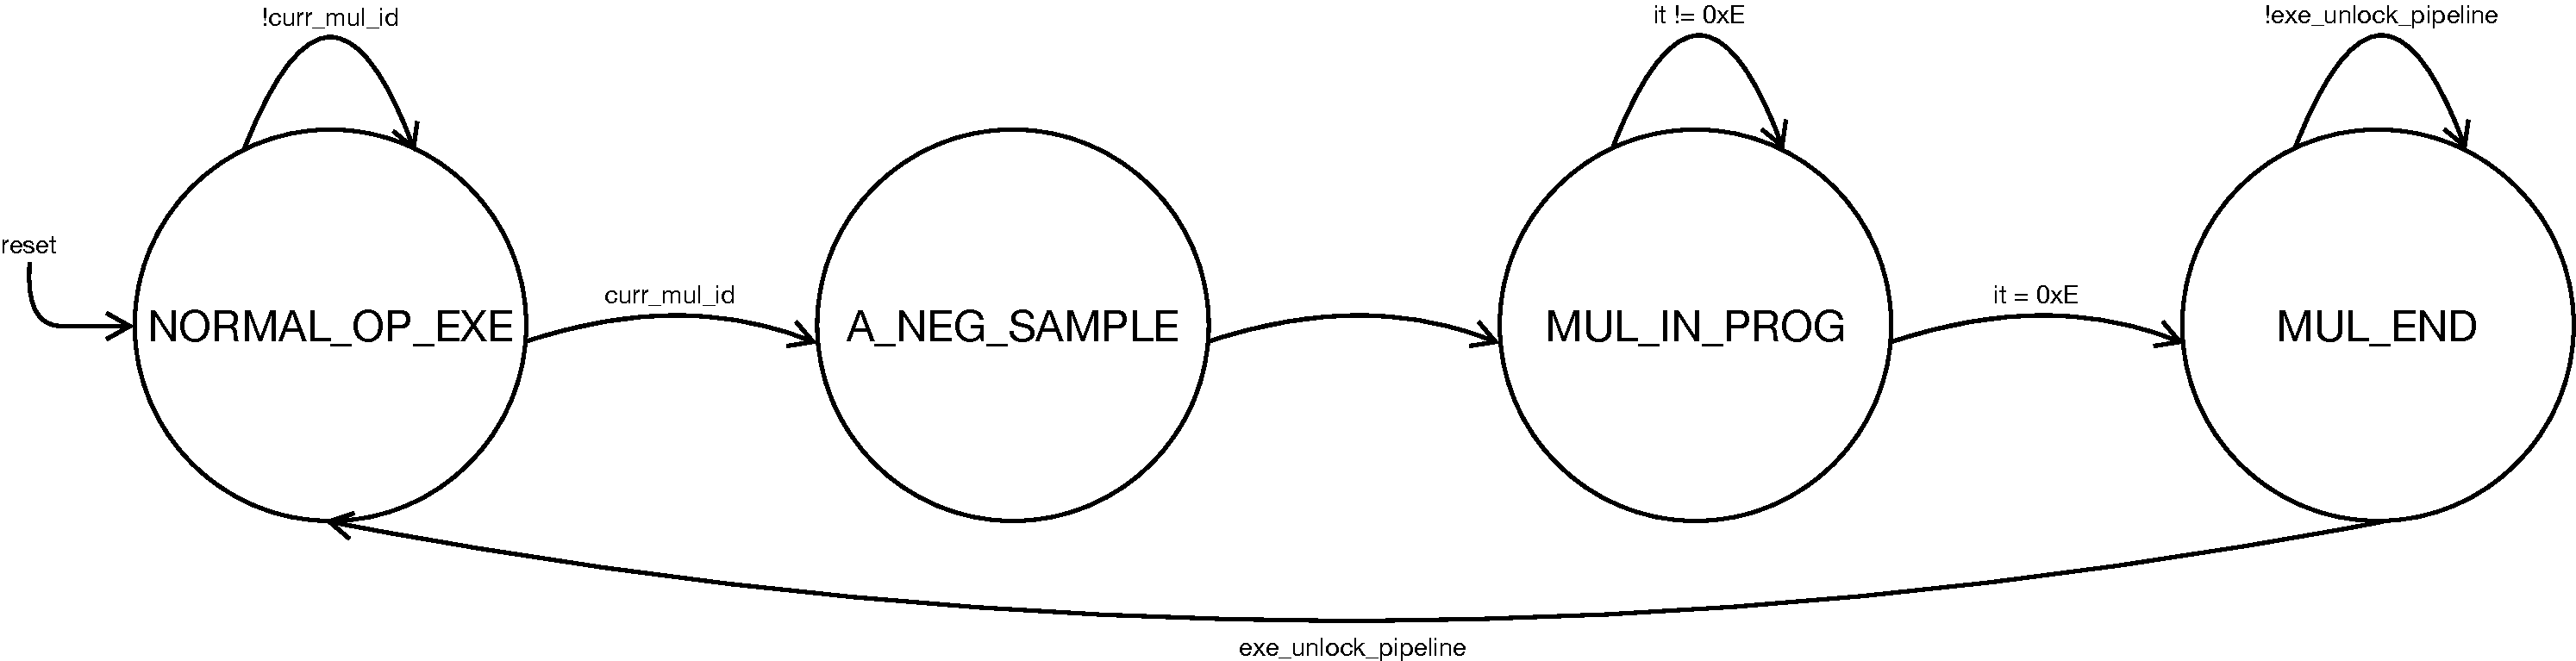
\includegraphics[width=\linewidth]{./chapters/figures/mul_fsm.pdf}
    \caption{EXE stage state diagram}
    \label{fig:mul_fsm}
\end{figure}

\subsection{NORMAL\_OP\_EXE}

This is the reset state and also the one where all the operations but \verb|mul| are executed. Here few checks are executed, therefore to ease the reader's understanding we have provided a flow diagram,
shown in figure \ref{fig:normal_op_flow_diagram}.

\begin{figure}[!ht]
	\centering
	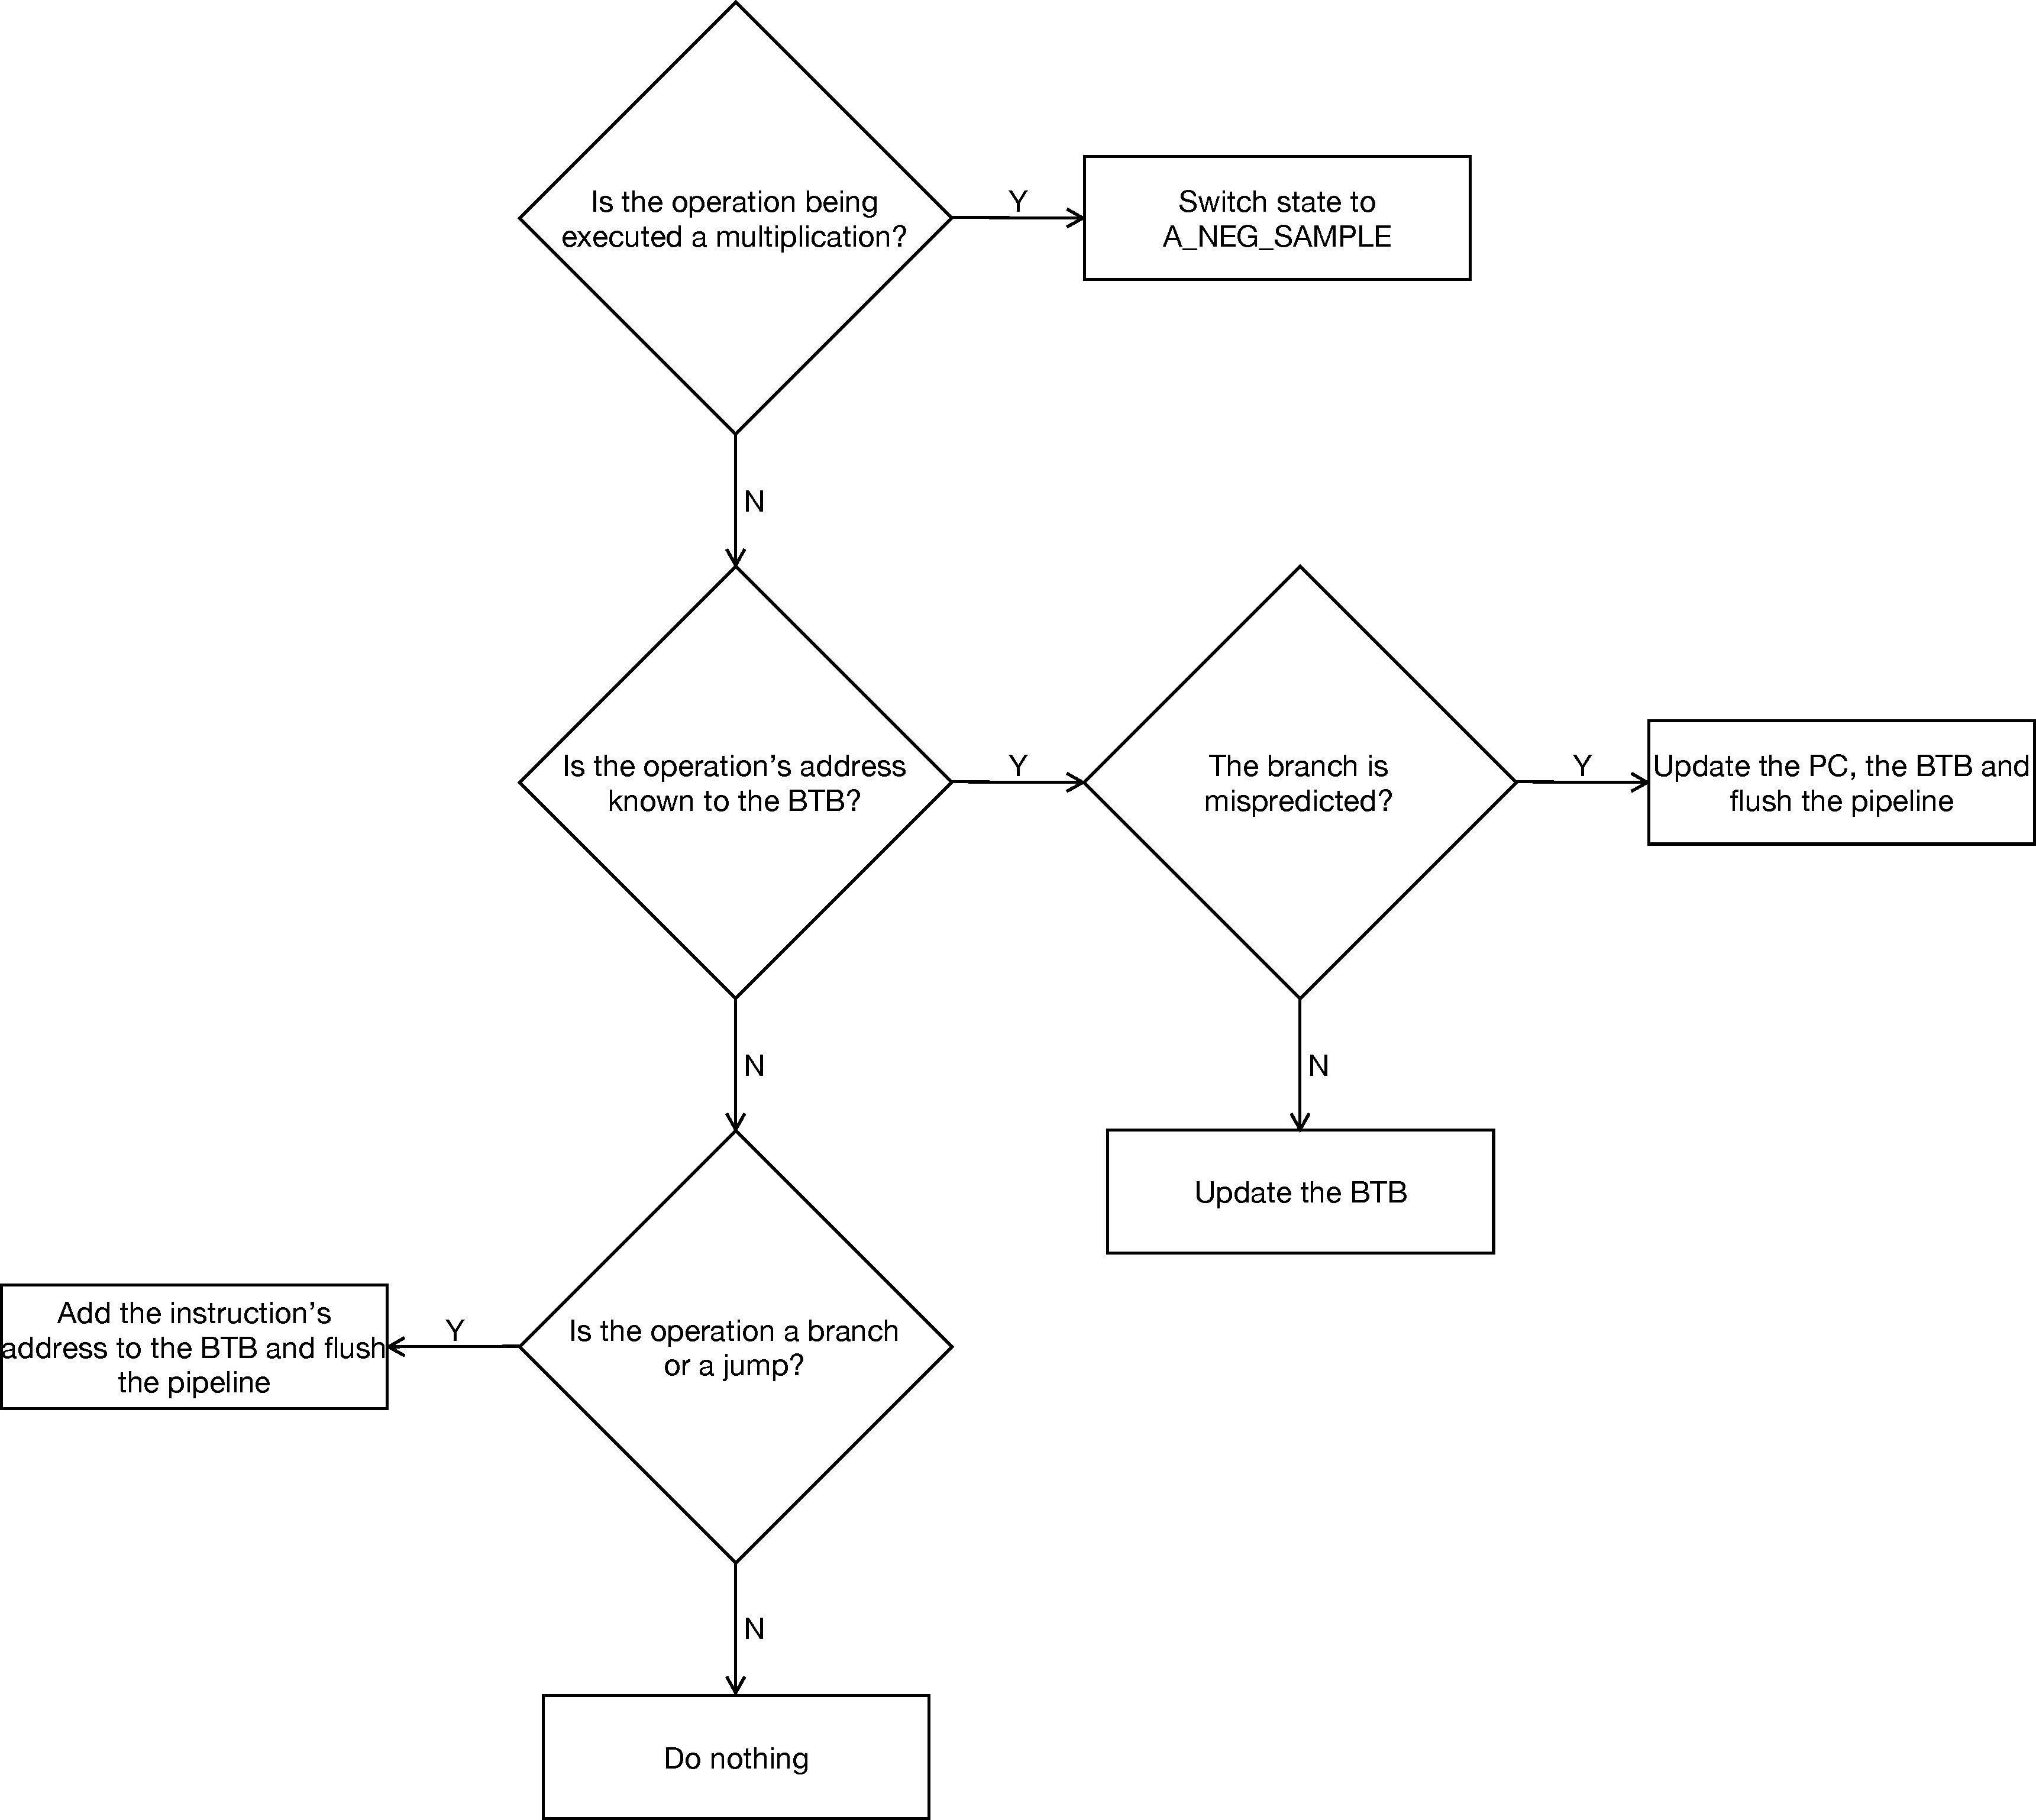
\includegraphics[width=\linewidth]{./chapters/figures/normal_op_diagram.pdf}
    \caption{NORMAL\_OP\_EXE flow diagram}
    \label{fig:normal_op_flow_diagram}
\end{figure}

The first check performed is whether the operation currently in the EXE stage is a multiplication or not. In the former case the EXE stage switch state as shown in figure \ref{fig:normal_op_flow_diagram} and stalls the pipeline,
while in the latter case the state remains unchanged. If the operation is not a multiplication, the other notable case is to check if the instruction is a branch or jump. To do so, it is controlled if the
BTB knew the instruction's address in the IF stage or not. If the address was known the only remaining check to be performed is whether the prediction was correct or not. In the first case the BTB prediction
is updated, otherwise besides the BTB's update the pipeline must be flushed and the PC changed.
If, instead, the address was not known, the FSM has to figure out if the instruction is a new branch or jump or not. In the latter case, besides writing as always the static control bits, nothing is done.
On the other hand, in the former case the address is added to the BTB, the pipeline is flushed and the PC is updated.

\subsection{A\_NEG\_SAMPLE}

This is the first state where the multiplication's execution starts. The EXE stage takes control over the ID/EXE registers, and uses the main adder to negate the value of the operand \verb|a| on 64 bits.
The next state of the FSM is automatically set to \verb|MUL_IN_PROG|.

\subsection{MUL\_IN\_PROG}

The FSM iterates over this state 15 times, using the multiplier's adder to calculate each time the partial result. As soon as the 15th iteration is executed, the next state is changed to \verb|MUL_END|.
In this state the EXE still controls the ID/EXE registers.

\subsection{MUL\_END}

This state is entered when the final result of the multiplication must be sampled by the EXE/MEM registers. After the result has been sampled, the EXE remains in this state (keeping therefore the pipeline locked)
until the multiplication result has reached the WB stage. When this happens, the next state of the FSM is set to \verb|NORMAL_OP_EXE| and the pipeline is unlocked.
Again, this shows a limitation of the \verb|mult|: its result cannot be forwarded to \verb|mflo| and \verb|mfhi| because it is on 64 bits and with out
forwarding logic only 32 bits can be forwarded. Hence, to maintain data flow correctness the multiplication's result must be sampled in the RF before the next instruction can enters the EXE stage.

\section{MEM stage}
\label{sec:cache_handling}

This stage, as all the previous ones, sends the static control bits to the datapath. When operations different from loads and stores pass through this stage, nothing more is done. Special attention must be
given to stores and, more importantly, to loads. In fact, the formers may generate cache evictions, while the latter ones may generate cache misses. Thanks to the design of the data cache and of the memory controller
cache eviction do not cause stalls, but cache misses do. Therefore, also in the MEM stage a FSM exists, of which the state diagram is shown in figure \ref{fig:mem_fsm}.

\begin{figure}[!ht]
	\centering
	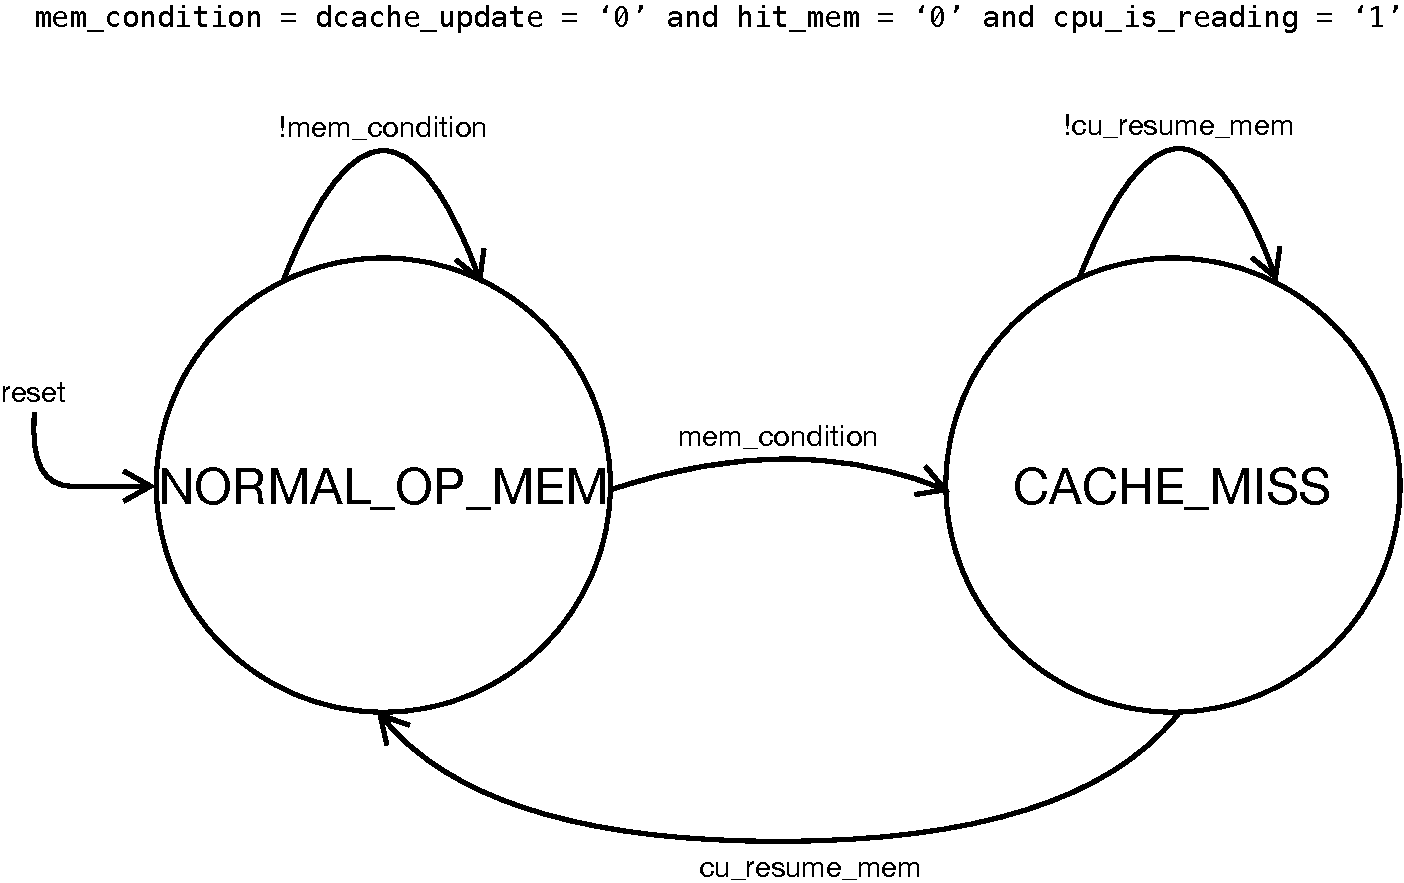
\includegraphics[width=0.5\linewidth]{./chapters/figures/mem_fsm.pdf}
    \caption{MEM stage state diagram}
    \label{fig:mem_fsm}
\end{figure}

\subsection{NORMAL\_OP\_MEM}

The FSM starts in this state and remains always here for all operations but loads. When a load is executed, the content indexed by the address may have been swapped out in cache, so the cache's \verb|hit| signal
would stay at 0. When this situation is detected, the MEM stage along with the stall unit stalls the entire processor and then sets the next state to \verb|CACHE_MISS|.

It is important to outline why \verb|mem_condition| in figure \ref{fig:mem_fsm} has that equation. Technically to detect the cache miss it would have been enough to look for \verb|dcache_update = 0 AND hit_mem = 0|, since
\verb|dcache_update| signals the processor's will to perform a read (by not updating anything in the memory) and \verb|hit_mem| signals if a hit or a miss have occurred. This is not sufficient however, because the cache is
accessed at every cycle using as address the output of the ALU, no matter if the instruction was actually a load or not. For this reason in the CW there is a field called \verb|cpu_is_reading|, which is set to 1 when the
processor wants to actually access the cache.

\subsection{CACHE\_MISS}
\label{subsec:cache_miss}

In this state the control unit hands over the control of the cache to the memory controller, which has recognized as well the cache miss in the previous cycle, by putting in high impedance \verb|dcache_update| and \verb|update_type_mem|.
The CU remains in this state as long as the memory controller does not raise the \verb|cu_resume| signal. When this happens, the pipeline is unlocked and the MEM stage FSM enters again the \verb|NORMAL_OP_MEM| state.

\subsubsection{Memory controller}

The memory controller resides outside the control unit. It acts as a communication layer for the cache and the RAM, moreover as said before is capable of resolving cache misses. It has its own FSM to perform its job,
shown in figure \ref{fig:memcontroller_fsm}.

\begin{figure}[!ht]
	\centering
	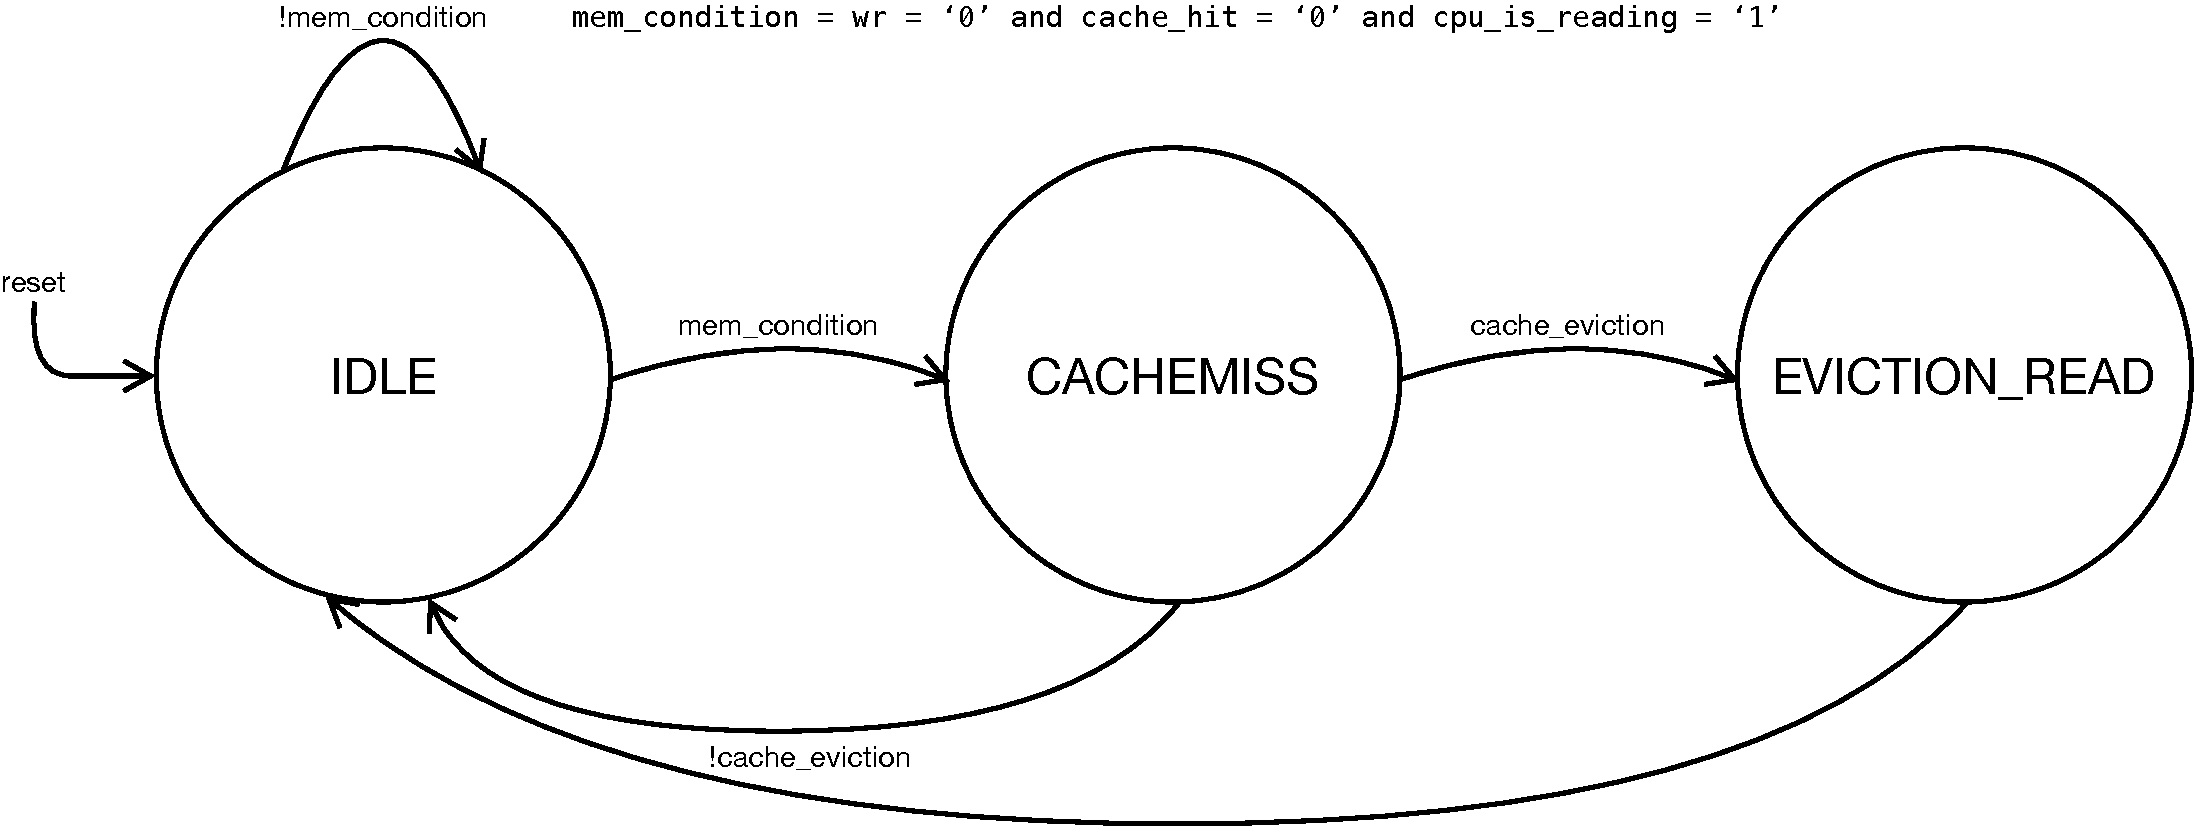
\includegraphics[width=0.8\linewidth]{./chapters/figures/memcontroller_fsm.pdf}
    \caption{Memory controller state diagram}
    \label{fig:memcontroller_fsm}
\end{figure}

\begin{enumerate}
    \item \verb|IDLE|: this is the reset state. It stays here as long as no cache miss is detected and it keeps its cache's control signal in high impedance.
    \item \verb|CACHEMISS|: in this state it asks the cache to update its value. Two possible outcomes are possible here: if the cache is not signalling the need of an eviction the next state will be \verb|IDLE|,
    otherwise it will be \verb|EVICTION_READ|. In this case the \verb|enable| signal of an internal register is enabled to sample the evicted data coming from the cache. In any case, after this state the control unit
    regains the cache's control.

    \item \verb|EVICTION_READ|: in this state the RAM is updated with the evicted data, then the next state is set to \verb|IDLE|. 
\end{enumerate}

In the \verb|IDLE| state, the memory controller may detect the occurrence of a data eviction during a write operation. This does not require a stall since it is able to directly forward the evicted data to the RAM.

\section{WB stage}

This is the final stage of the pipeline. Its job is fairly easy, since it has to forward the control signals to the datapath without any special exception. Besides this, the only other thing it does is to unlock
the pipeline when a multiplication has reached this stage.

\section{Stall unit}
\label{sec:stall_unit}

The stall unit has the duty of detecting data hazards and of handling all the signals required to stall the processor when needed. Hazards are detected by looking at \verb|rs| and \verb|rt| stored in the
ID/EXE registers, and by confronting them with the \verb|rd| registers stored in the EXE/MEM and MEM/WB registers. The \verb|rd| registers are accompanied in the pipeline by a bit that specifies whether
they are valid or not. This is necessary because to reduce the switching activity the registers not needed by an operation are disabled, therefore an invalid hazard could be detected.
Data hazards are actually checked also from the ID stage, because as said in section \ref{sec:cu_exe_stage} if a multiplication detects an hazard it has to stall.

This unit, before attempting to forward data, checks if it has to stall because the control unit has requested so. The sources of a stall can be:

\begin{enumerate}
    \item A cache miss has occurred. This has the highest priority in the stall unit to guarantee data correctness. For example, a load could trigger a cache miss while a multiplication enters the EXE stage:
    if they have been served in the reversed order, the load would store in the register file the wrong data.

    \item A multiplication is in the EXE stage. In this case \verb|nop| operations are scheduled from the MEM stage onwards in order to allow to the operations in the MEM and WB stage to complete their execution.
    
    \item A multiplication is in the ID stage and a data hazard has been detected. 
\end{enumerate}

If none of the above conditions are verified, the stall unit then controls what data can forwards to the EXE stage. Not all operations supports forwarding, as in the case of a \verb|j|, or they could support the
forwarding only of the \verb|rs| register, as in the case of most |I| instructions. This information is embedded in the CW of the instruction in the EXE stage and it is encoded in two bits. The possible values are:

\begin{enumerate}
    \item \verb|00|: forwarding is not supported.
    \item \verb|01|: only \verb|rs| can be forwarded.
    \item \verb|10|: both \verb|rs| and \verb|rt| can be forwarded (\verb|rt| goes inside the adder's and shifter's operands).
    \item \verb|11|: both \verb|rs| and \verb|rt| can be forwarded (\verb|rt| is forwarded in \verb|op_b|, the signal where the data to be saved in the cache during a store is kept).
\end{enumerate}

When the forwarding is supported by the instruction, it could be possible to generate a stall. In fact, if the instruction that should forward the data is a load, and said load is the MEM stage,
it has not fetched yet the content of the memory. In this situation a bubble must be inserted in the pipeline.
\chapter{Simulation, Synthesis and Implementation}
\label{chap:syn_impl}

In this chapter we will discuss the flow we have followed from the DLX's simulation to implementation.

\section{Simulation}

The simulation has been performed on two tools: {\it Vivado} and {\it ModelSim}. The various components of the DLX have been developed
by using the former tool, which is also the one we used to perform unit testing. The latter has been used to perform the final integration
testing. In the {\it dlx\_sim} folder a simulation script for ModelSim can be found, called \verb|sim_script.tcl|.

This script first lets ModelSim to analyze the various VHDL files, then analyzed one of the provided testbenches and it runs a simulation
for 100 ns.

We did not provided the testbenches we have written for testing the components in isolation because, during the final tests, we had to change
many small things and we did not have enough time to modify them as well.

\subsection{Test files}

In the folder {\it tb} all the testbenches that can be used with \verb|sim_script.tcl| are stored. By running all the scripts we have provided
it is possible to verify the correctness of the entire DLX's ISA.

The files are:
\begin{enumerate}
    \item \verb|tb_arith.vhd|: it aims at testing all the various arithmetic instructions, either of type R and I, by also the forwarding logic.
    \item \verb|tb_branches.vhd|: it tests all the branches executed by the DLX along with the prediction abilities of the BTB.
    \item \verb|tb_jalr.vhd|: it verifies the correctness of the \verb|jalr| instruction. This test is separated because otherwise \verb|tb_branches| would have been too big.
    \item \verb|tb_jump_and_link.vhd|: it shows the ability of the processor to follows the ABI and to execute the \verb|jalr| instruction. As a bonus, it demonstrate the ability of the control unit and memory controller to handle cache misses.
    \item \verb|tb_load_store.vhd|: it tests if the processor is capable to handle all the supported loads and stores.
    \item \verb|tb_mult.vhd|: it tests if the multiplication is properly executed in various scenarios, like when it would need forwarding and if it stalls the pipeline correctly.
    \item \verb|tb_r.vhd|: it checks whether the processor is able to execute all the supported R instructions, with and without forwarding.
\end{enumerate}

The related assembly files can be found in the folder {\it test\_assembly}.

\section{Synthesis}

Each time we developed a new datapath component, we have synthetized it to assess if it was able to meet our initial frequency target of $1\ GHz$. Among all the datapath components,
the multiplier was the only one to not meet such standard, as it is able to reach a little bit more than $850\ MHz$ if synthetized alone.
When we synthetized the first version of the complete DLX (that is, also with the control unit and the memory controller) we used the \verb|set_dont_touch| command to

\begin{enumerate}
    \item use \verb|compile_ultra| on critical parts of the design, that is the EXE stage and the control unit;
    \item use \verb|compile| on the rest of the processor, as it less time-sensitive.
\end{enumerate}

The \verb|set_dont_touch| command, in fact, tells to the tool to not modify anymore an elaborated and compiled entity. This removes some optimization opportunities, but it is very handy
when dealing with big circuits such as a processor to reduce the synthesis time.
The result of the synthesis didn't meet our performance target, since it reached only $800 MHz$, but we still were satisfied. However, the more we have tested the DLX, the more we have found
issues that needed to be fixed. Most of the issue were related to the control unit and the stall management, therefore it would have needed a complete redesign. Unfortunately, there was not enough
time to do it, therefore we have been forced to add some hacks to make it work. This has severely affected the DLX's overall performance, as $t_{CK}$ had to be raised to $1.9\ ns$. This results in
$f_{CK} \approx 525\ MHz$, which is almost half of our initial frequency target. This value has been obtained by synthetizing the whole DLX with the \verb|compile_ultra| command.

Below, the final time, area and power report are shown.

\subsection{Time report}

\begin{verbatim}
Startpoint: ctrl_u/curr_es_reg[1]
            (rising edge-triggered flip-flop clocked by clk)
  Endpoint: dp/id_exe_regs/b_mult_reg/curr_data_reg[23]
            (rising edge-triggered flip-flop clocked by clk)
  Path Group: clk
  Path Type: max

  Des/Clust/Port     Wire Load Model       Library
  ------------------------------------------------
  dlx_syn            5K_hvratio_1_1        NangateOpenCellLibrary

  Point                                                   Incr       Path
  --------------------------------------------------------------------------
  clock clk (rise edge)                                   0.00       0.00
  clock network delay (ideal)                             0.00       0.00
  ctrl_u/curr_es_reg[1]/CK (DFF_X1)                       0.00       0.00 r
  ctrl_u/curr_es_reg[1]/Q (DFF_X1)                        0.09       0.09 r
  U4305/ZN (NAND3_X1)                                     0.04       0.13 f
  U4627/ZN (NAND2_X1)                                     0.04       0.17 r
  U4054/ZN (AND4_X2)                                      0.07       0.23 r
  U4596/ZN (NAND4_X1)                                     0.05       0.29 f
  U3980/ZN (NOR2_X2)                                      0.07       0.36 r
  U3938/Z (BUF_X2)                                        0.05       0.41 r
  U4032/ZN (INV_X1)                                       0.04       0.45 f
  U7477/ZN (OAI22_X1)                                     0.05       0.50 r
  U7153/ZN (INV_X1)                                       0.02       0.52 f
  U7151/ZN (NAND2_X1)                                     0.03       0.55 r
  U4560/ZN (XNOR2_X1)                                     0.07       0.62 r
  U4341/ZN (NOR2_X1)                                      0.03       0.65 f
  U4558/ZN (NOR2_X1)                                      0.07       0.72 r
  U4550/ZN (NAND2_X1)                                     0.04       0.76 f
  U4549/ZN (NOR2_X1)                                      0.05       0.80 r
  U4529/ZN (AOI21_X1)                                     0.03       0.84 f
  U4466/ZN (INV_X1)                                       0.06       0.90 r
  U4459/ZN (AOI21_X1)                                     0.05       0.95 f
  U4323/ZN (OAI21_X1)                                     0.05       1.00 r
  U4322/ZN (XNOR2_X1)                                     0.06       1.06 r
  U4319/ZN (NAND2_X1)                                     0.03       1.09 f
  U4317/ZN (NOR2_X1)                                      0.04       1.13 r
  U3971/ZN (AND4_X2)                                      0.07       1.20 r
  U4452/ZN (NAND2_X1)                                     0.03       1.23 f
  U4450/ZN (AND2_X1)                                      0.04       1.27 f
  U4316/ZN (OAI21_X1)                                     0.04       1.32 r
  U4315/ZN (NAND2_X1)                                     0.04       1.35 f
  U4314/ZN (NAND2_X1)                                     0.04       1.40 r
  U3973/ZN (OR2_X2)                                       0.05       1.44 r
  U4443/ZN (AND2_X1)                                      0.04       1.48 r
  U4390/ZN (NAND2_X1)                                     0.04       1.52 f
  U4004/ZN (NAND2_X1)                                     0.06       1.59 r
  U6576/ZN (NAND2_X1)                                     0.07       1.66 f
  U4137/ZN (NOR2_X1)                                      0.11       1.77 r
  U3277/ZN (AOI22_X1)                                     0.05       1.82 f
  U3278/ZN (NAND3_X1)                                     0.04       1.86 r
  dp/id_exe_regs/b_mult_reg/curr_data_reg[23]/D (DFF_X1)
                                                          0.01       1.87 r
  data arrival time                                                  1.87

  clock clk (rise edge)                                   1.90       1.90
  clock network delay (ideal)                             0.00       1.90
  dp/id_exe_regs/b_mult_reg/curr_data_reg[23]/CK (DFF_X1)
                                                          0.00       1.90 r
  library setup time                                     -0.03       1.87
  data required time                                                 1.87
  --------------------------------------------------------------------------
  data required time                                                 1.87
  data arrival time                                                 -1.87
  --------------------------------------------------------------------------
  slack (MET)                                                        0.00
\end{verbatim}

As it can be seen, the critical path starts in the EXE part of the control unit, specifically from the register that holds the EXE FSM's state,
and terminates in the multiplication's register \verb|b| data.

\subsection{Area report}

\begin{verbatim}
Number of ports:                          600
Number of nets:                          6868
Number of cells:                         5918
Number of combinational cells:           5083
Number of sequential cells:               832
Number of macros:                           0
Number of buf/inv:                        899
Number of references:                      54

Combinational area:       10821.944148
Noncombinational area:    8594.991691
Net Interconnect area:      undefined  (Wire load has zero net area)

Total cell area:          19416.935839
Total area:                 undefined
\end{verbatim}

\subsection{Power report}

\begin{verbatim}
Global Operating Voltage = 1.1  
Power-specific unit information :
    Voltage Units = 1V
    Capacitance Units = 1.000000ff
    Time Units = 1ns
    Dynamic Power Units = 1uW    (derived from V,C,T units)
    Leakage Power Units = 1nW


  Cell Internal Power  =   6.9865 mW   (80%)
  Net Switching Power  =   1.7389 mW   (20%)
                         ---------
Total Dynamic Power    =   8.7254 mW  (100%)

Cell Leakage Power     = 463.1583 uW


                 Internal         Switching           Leakage            Total
Power Group      Power            Power               Power              Power   (   %    )  Attrs
--------------------------------------------------------------------------------------------------
io_pad             0.0000            0.0000            0.0000            0.0000  (   0.00%)
memory             0.0000            0.0000            0.0000            0.0000  (   0.00%)
black_box          0.0000            0.0000            0.0000            0.0000  (   0.00%)
clock_network     11.1759        1.1986e+03          114.8263        1.2098e+03  (  13.17%)
register       6.7667e+03           72.8469        1.4489e+05        6.9844e+03  (  76.01%)
sequential         0.0000            0.0000            0.0000            0.0000  (   0.00%)
combinational    208.6468          467.4612        3.1815e+05          994.2623  (  10.82%)
--------------------------------------------------------------------------------------------------
Total          6.9865e+03 uW     1.7389e+03 uW     4.6316e+05 nW     9.1886e+03 uW
\end{verbatim}

\subsection{Synthesis files}

The synthesis file are stored in the {\it dlx\_syn} folder. Inside the folder it is provided a script called
\verb|syn_script.tcl|, capable of running the the whole synthesis process.

\section{Implementation}
\chapter{Conclusions}
\label{chap:conclusions}

All in all, we have mixed feelings for this project. For a part we are satisfied by the amount of things we have been able to achieve,
since we managed to add a large instruction set, a BTB, two caches, the forwarding unit and the ABI support.

However, we regret the way we implemented the multiplier. Actually, we regret to have added it at all.

In the earliest phase
of development we have decided to rearrange the Booth's algorithm in such a way that it could be pipelined and would not take a lot of area.
Unfortunately, we did not have enough time to implement it properly and this forced us to do compromise in order to keep it, compromises we
would not have accepted by going back. It has hugely increased the complexity of the control unit and the amount of signals needed to handle
all the possible stalls and corner cases. It also took a lot of time from us for testing and it had many problems, time that we could have
dedicated to improve the rest of the system. This is all without even considering the fact that it is the only component in the EXE stage that,
synthesized by itself with \verb|compile_ultra|, is not able to reach the target frequency of $1\ GHz$.

The final frequency of our DLX is, indeed, "only" of $525\ MHz$, a decent value but far from our target. Sadly due to all the delays we had
we did not have time to remove it and test everything again so in the end we kept it.

% \input{./chapters/chap_name}
% and so on
%
%%%%%%%%%%%%%%%%%%%%%%%%%%%%%%%%%%%%%%%%%%%%%%%%%%%%%%
%    
% HERE IS WHERE YOU INCLUDE YOUR APPENDICES (IF ANY)
%
%\appendix
%%%% Appendix A
\chapter{Adder behavioural VHDL}
\label{appendix1}

	\lstinputlisting[language=VHDL, breaklines=true]{appendices/files/adder.vhd}

% \lstinputlisting is an alternative way to import text or code from an external file. In this example the behavioural VHDL description of an adder contained in the file adder.vhd is imported. 
% Note that you can set the language of the code that you want to import (VHDL in this example). When you set the language you will see the keywords of that specific language highlighted in your output pdf file.
%You can set a lot parameters: for some examples take a look at the chapter 'How to document the project' that can you find in DLX_Project.pdf.
% \input{./appendices/appendix2}
% and so on
%
%%%%%%%%%%%%%%%%%%%%%%%%%%%%%%%%%%%%%%%%%%%%%%%%%%%%%%

\printbibliography

\end{document}